\documentclass{exam}

\usepackage[utf8]{inputenc}
\usepackage{array}
\usepackage{graphicx}
\usepackage{caption}
\usepackage{float}

%\newcolumntype{L}[1]{>{\raggedright\let\newline\\\arraybackslash\hspace{0pt}}m{#1}}
\usepackage{amsmath}

\newcounter{eqn}
\renewcommand*{\theeqn}{\alph{eqn})}
\newcommand{\num}{\refstepcounter{eqn}\text{\theeqn}\;}


\makeatletter
\newcommand{\putindeepbox}[2][0.7\baselineskip]{{%
    \setbox0=\hbox{#2}%
    \setbox0=\vbox{\noindent\hsize=\wd0\unhbox0}
    \@tempdima=\dp0
    \advance\@tempdima by \ht0
    \advance\@tempdima by -#1\relax
    \dp0=\@tempdima
    \ht0=#1\relax
    \box0
}}
\makeatother


\title{Questionary}

\begin{document}

\maketitle
%\section*{Questionary}

\section*{Design}

\subsection*{Color Theme}

The following images show different color themes of a table, containing patient information. 
Red rows indicate that our algorithm detected a potential decubitus patient. 

\begin{tabular}{cc}
	\num\putindeepbox[7pt]{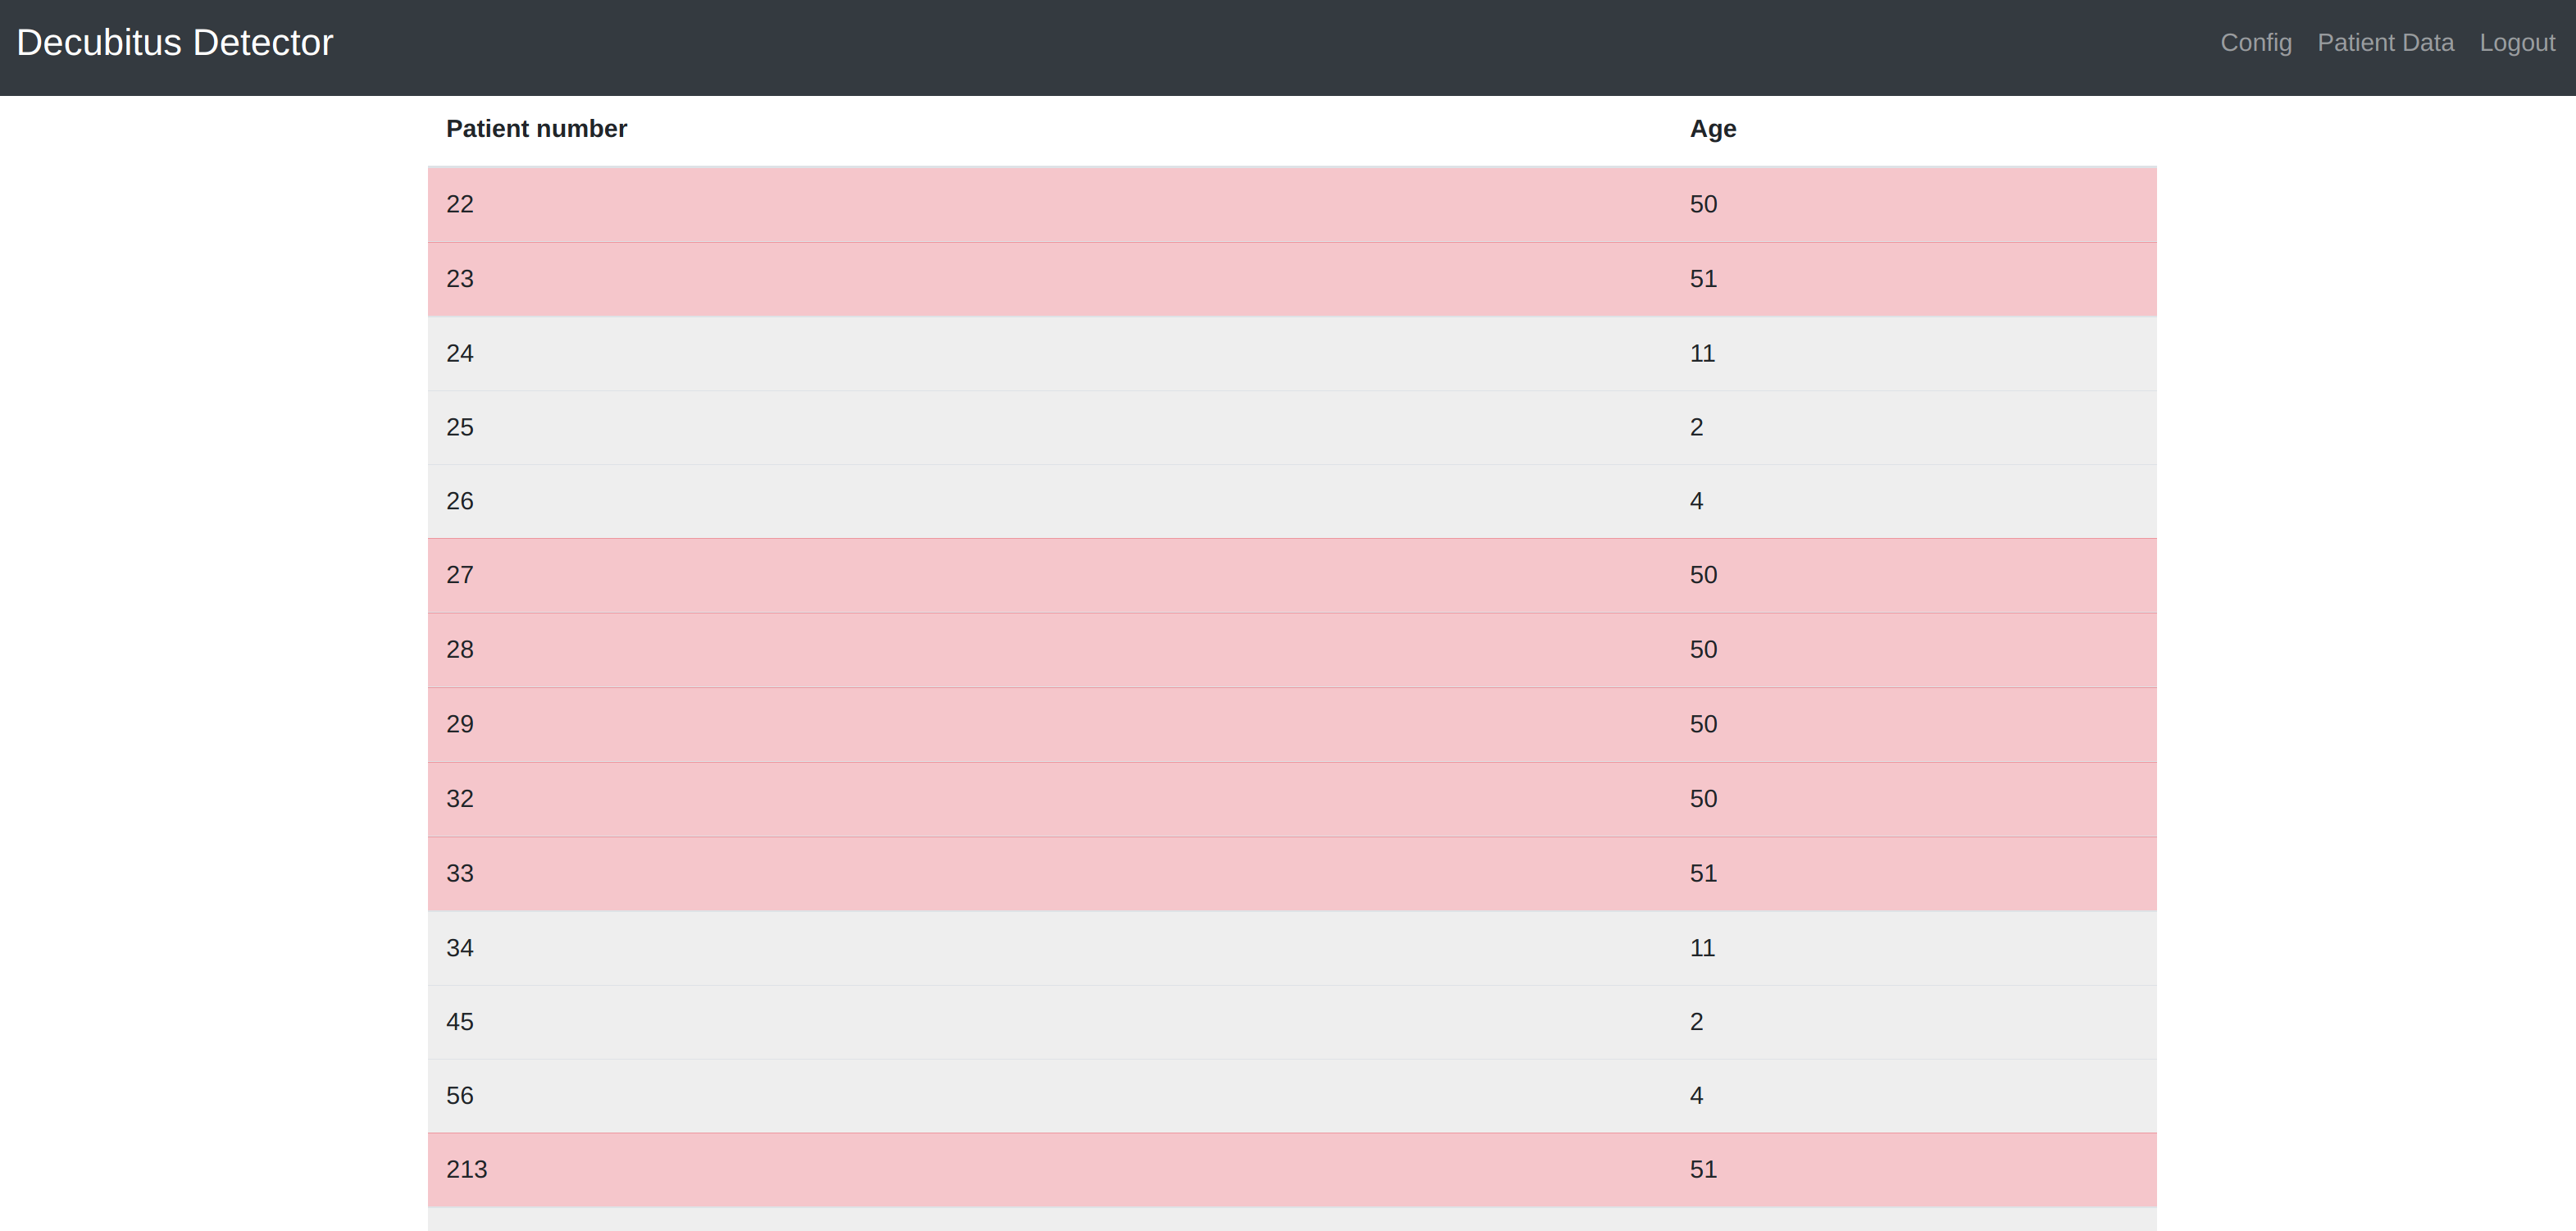
\includegraphics[width=0.45\linewidth]{images/gray.png}}
	& \num\putindeepbox[7pt]{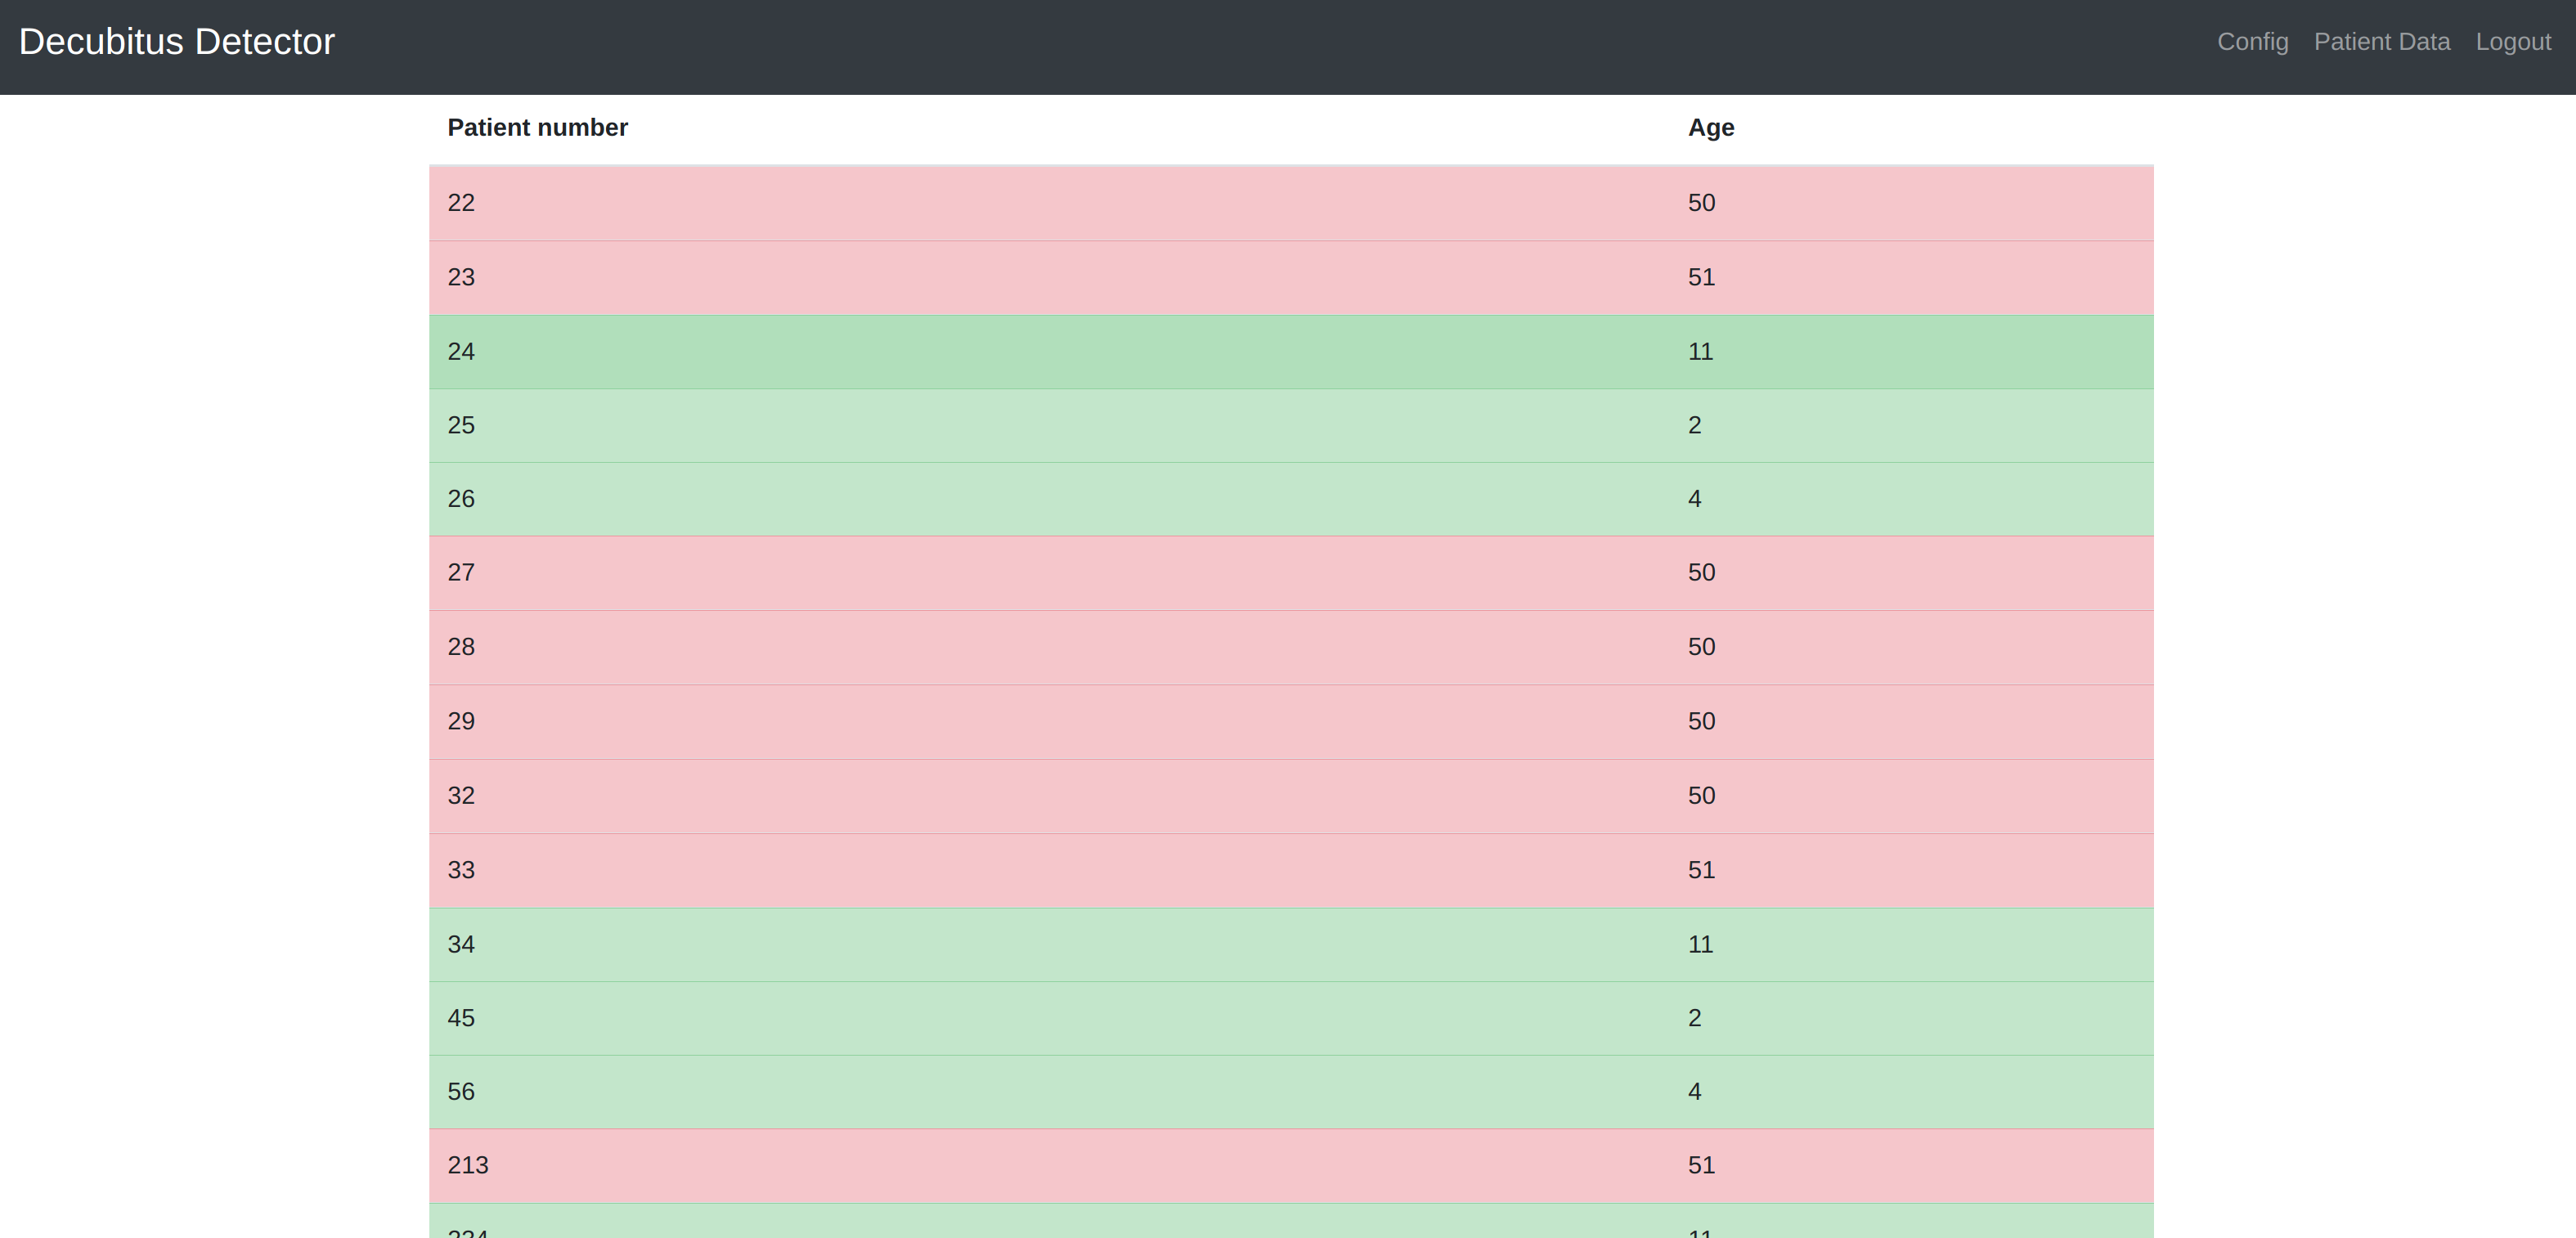
\includegraphics[width=0.45\linewidth]{images/green.png}} \\
	\num\putindeepbox[7pt]{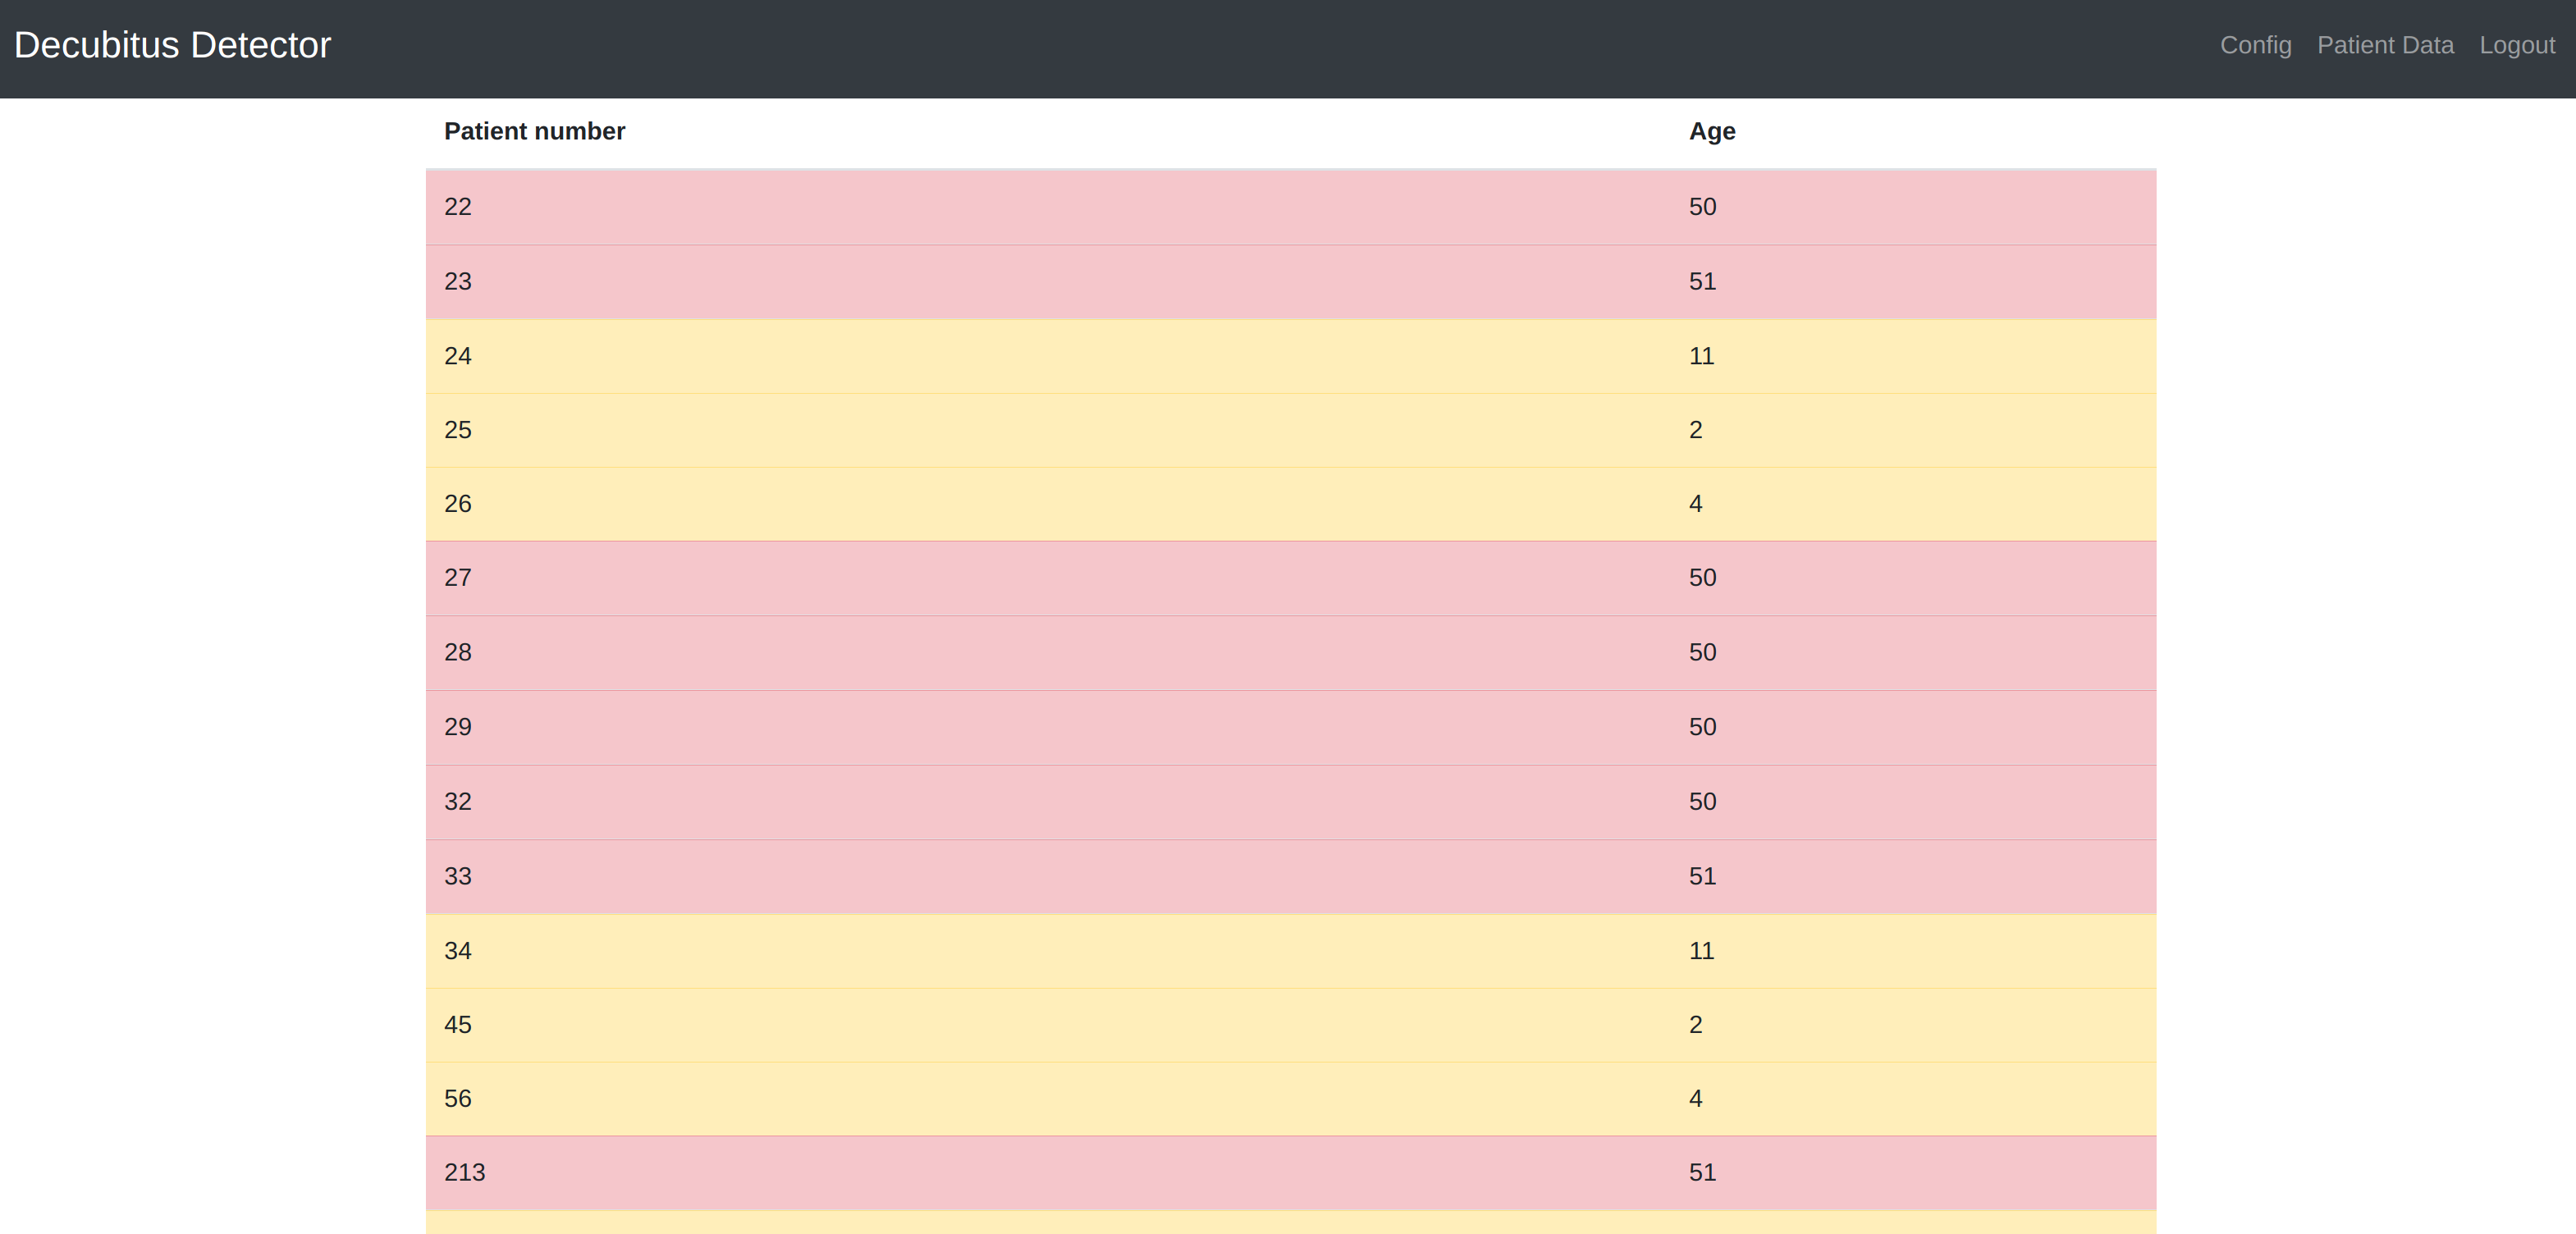
\includegraphics[width=0.45\linewidth]{images/yellow.png}}
	& \num\putindeepbox[7pt]{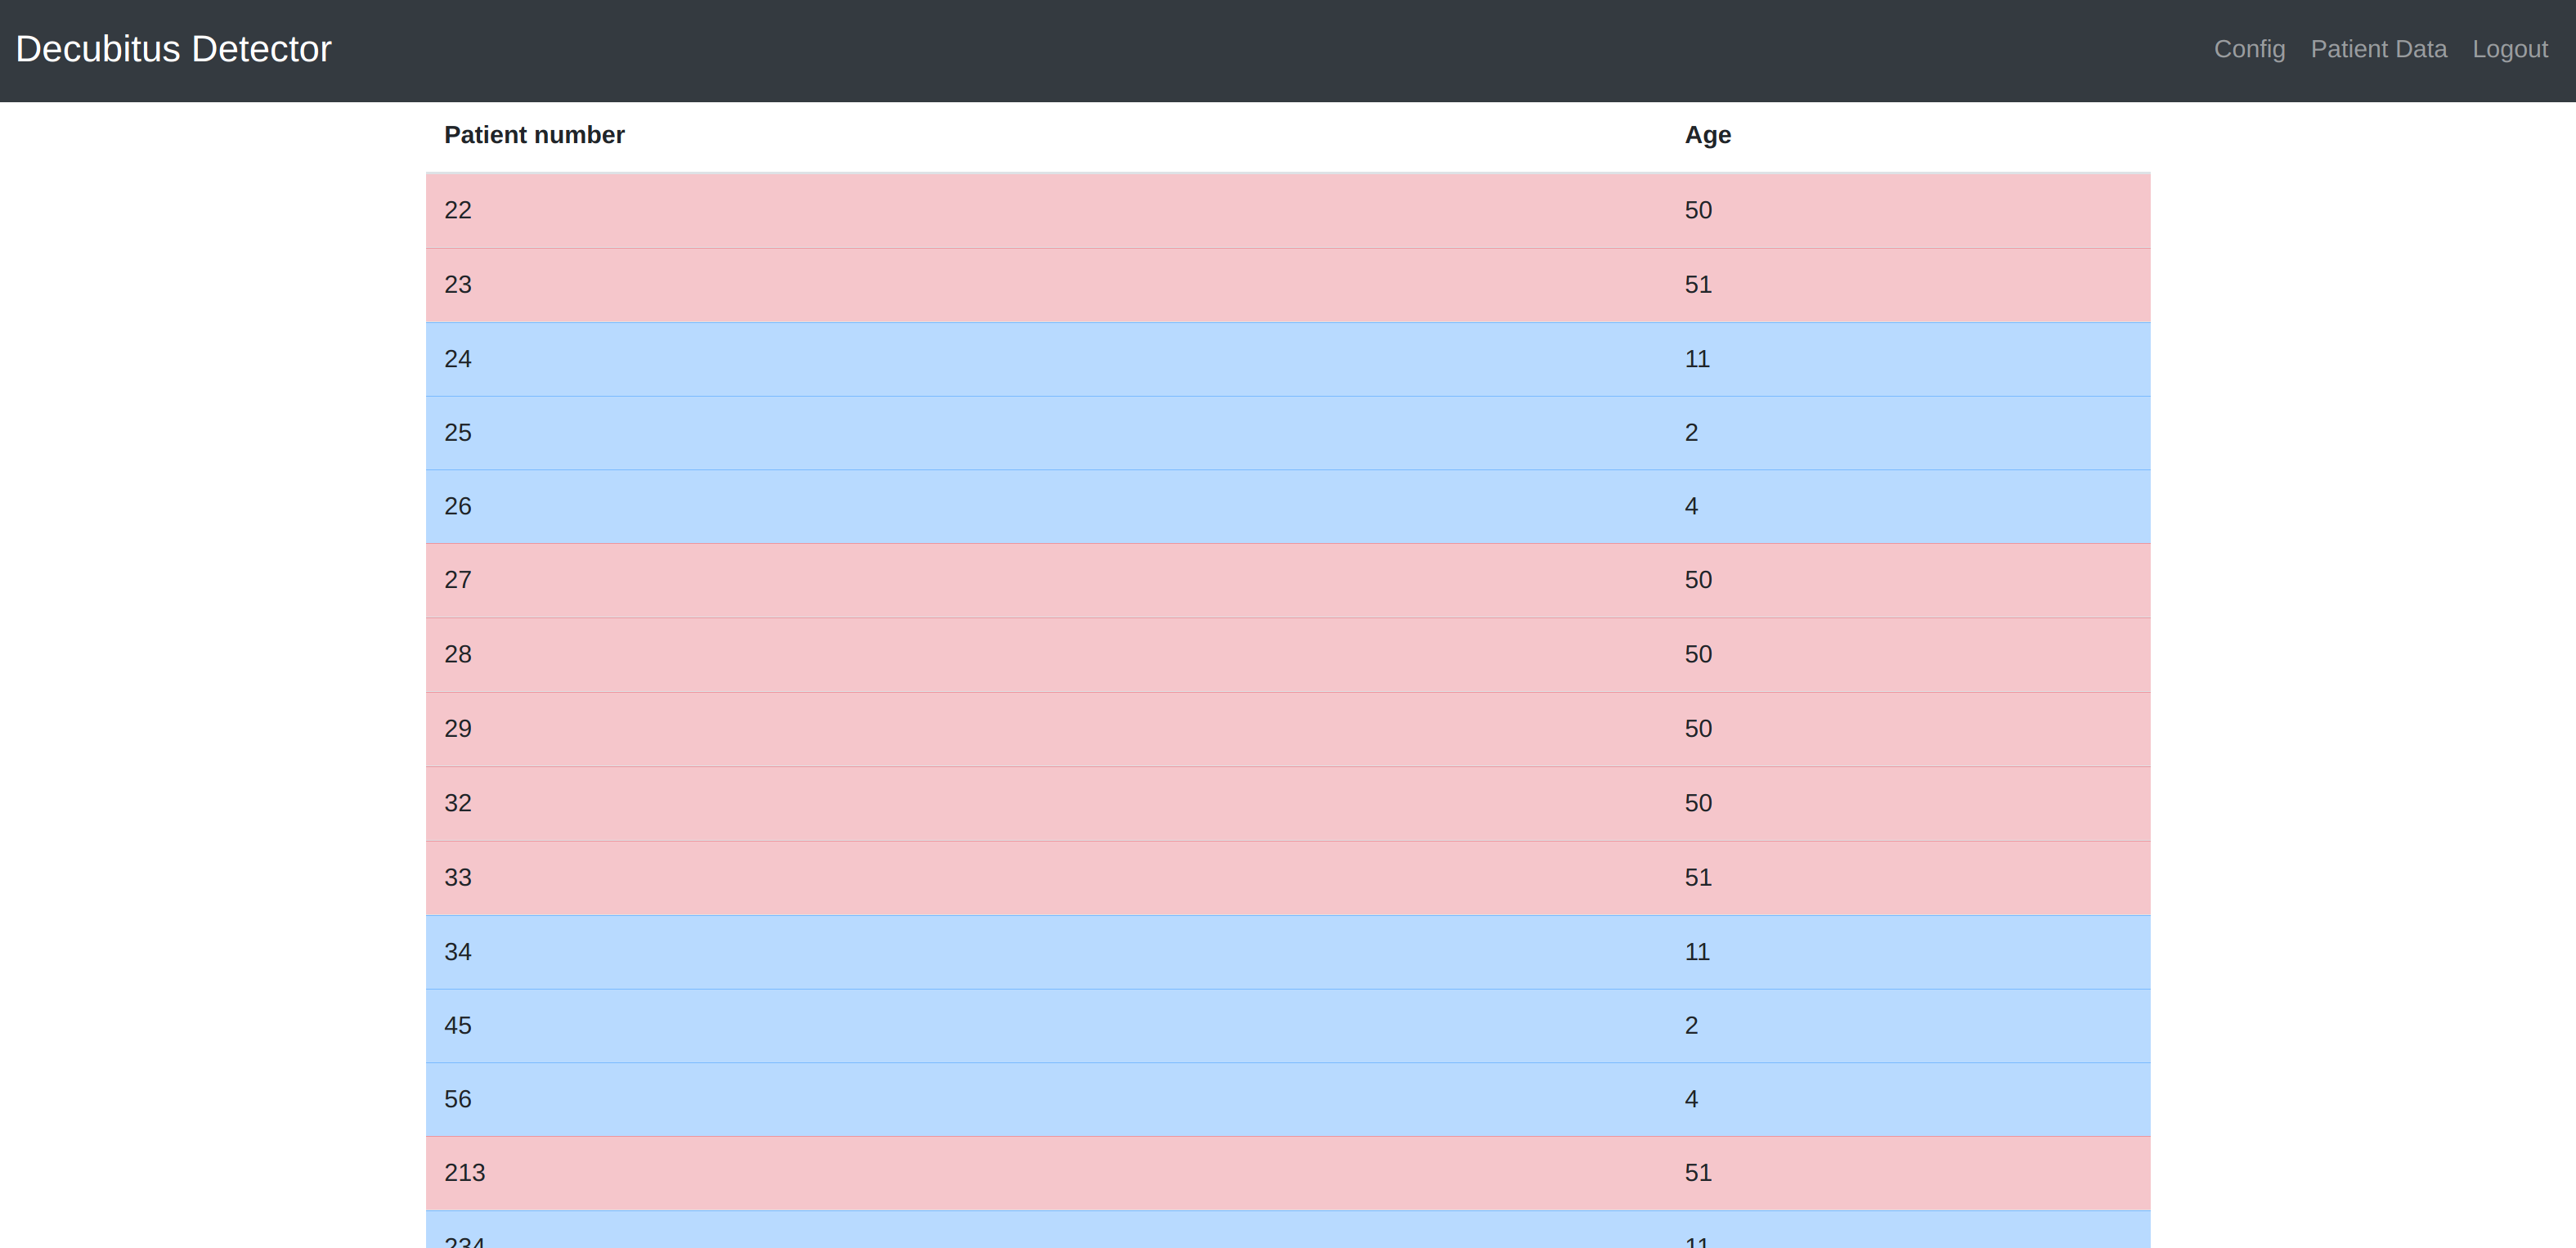
\includegraphics[width=0.45\linewidth]{images/blue.png}} \\
\end{tabular}


\iffalse
\begin{figure}[H]
	\centering
  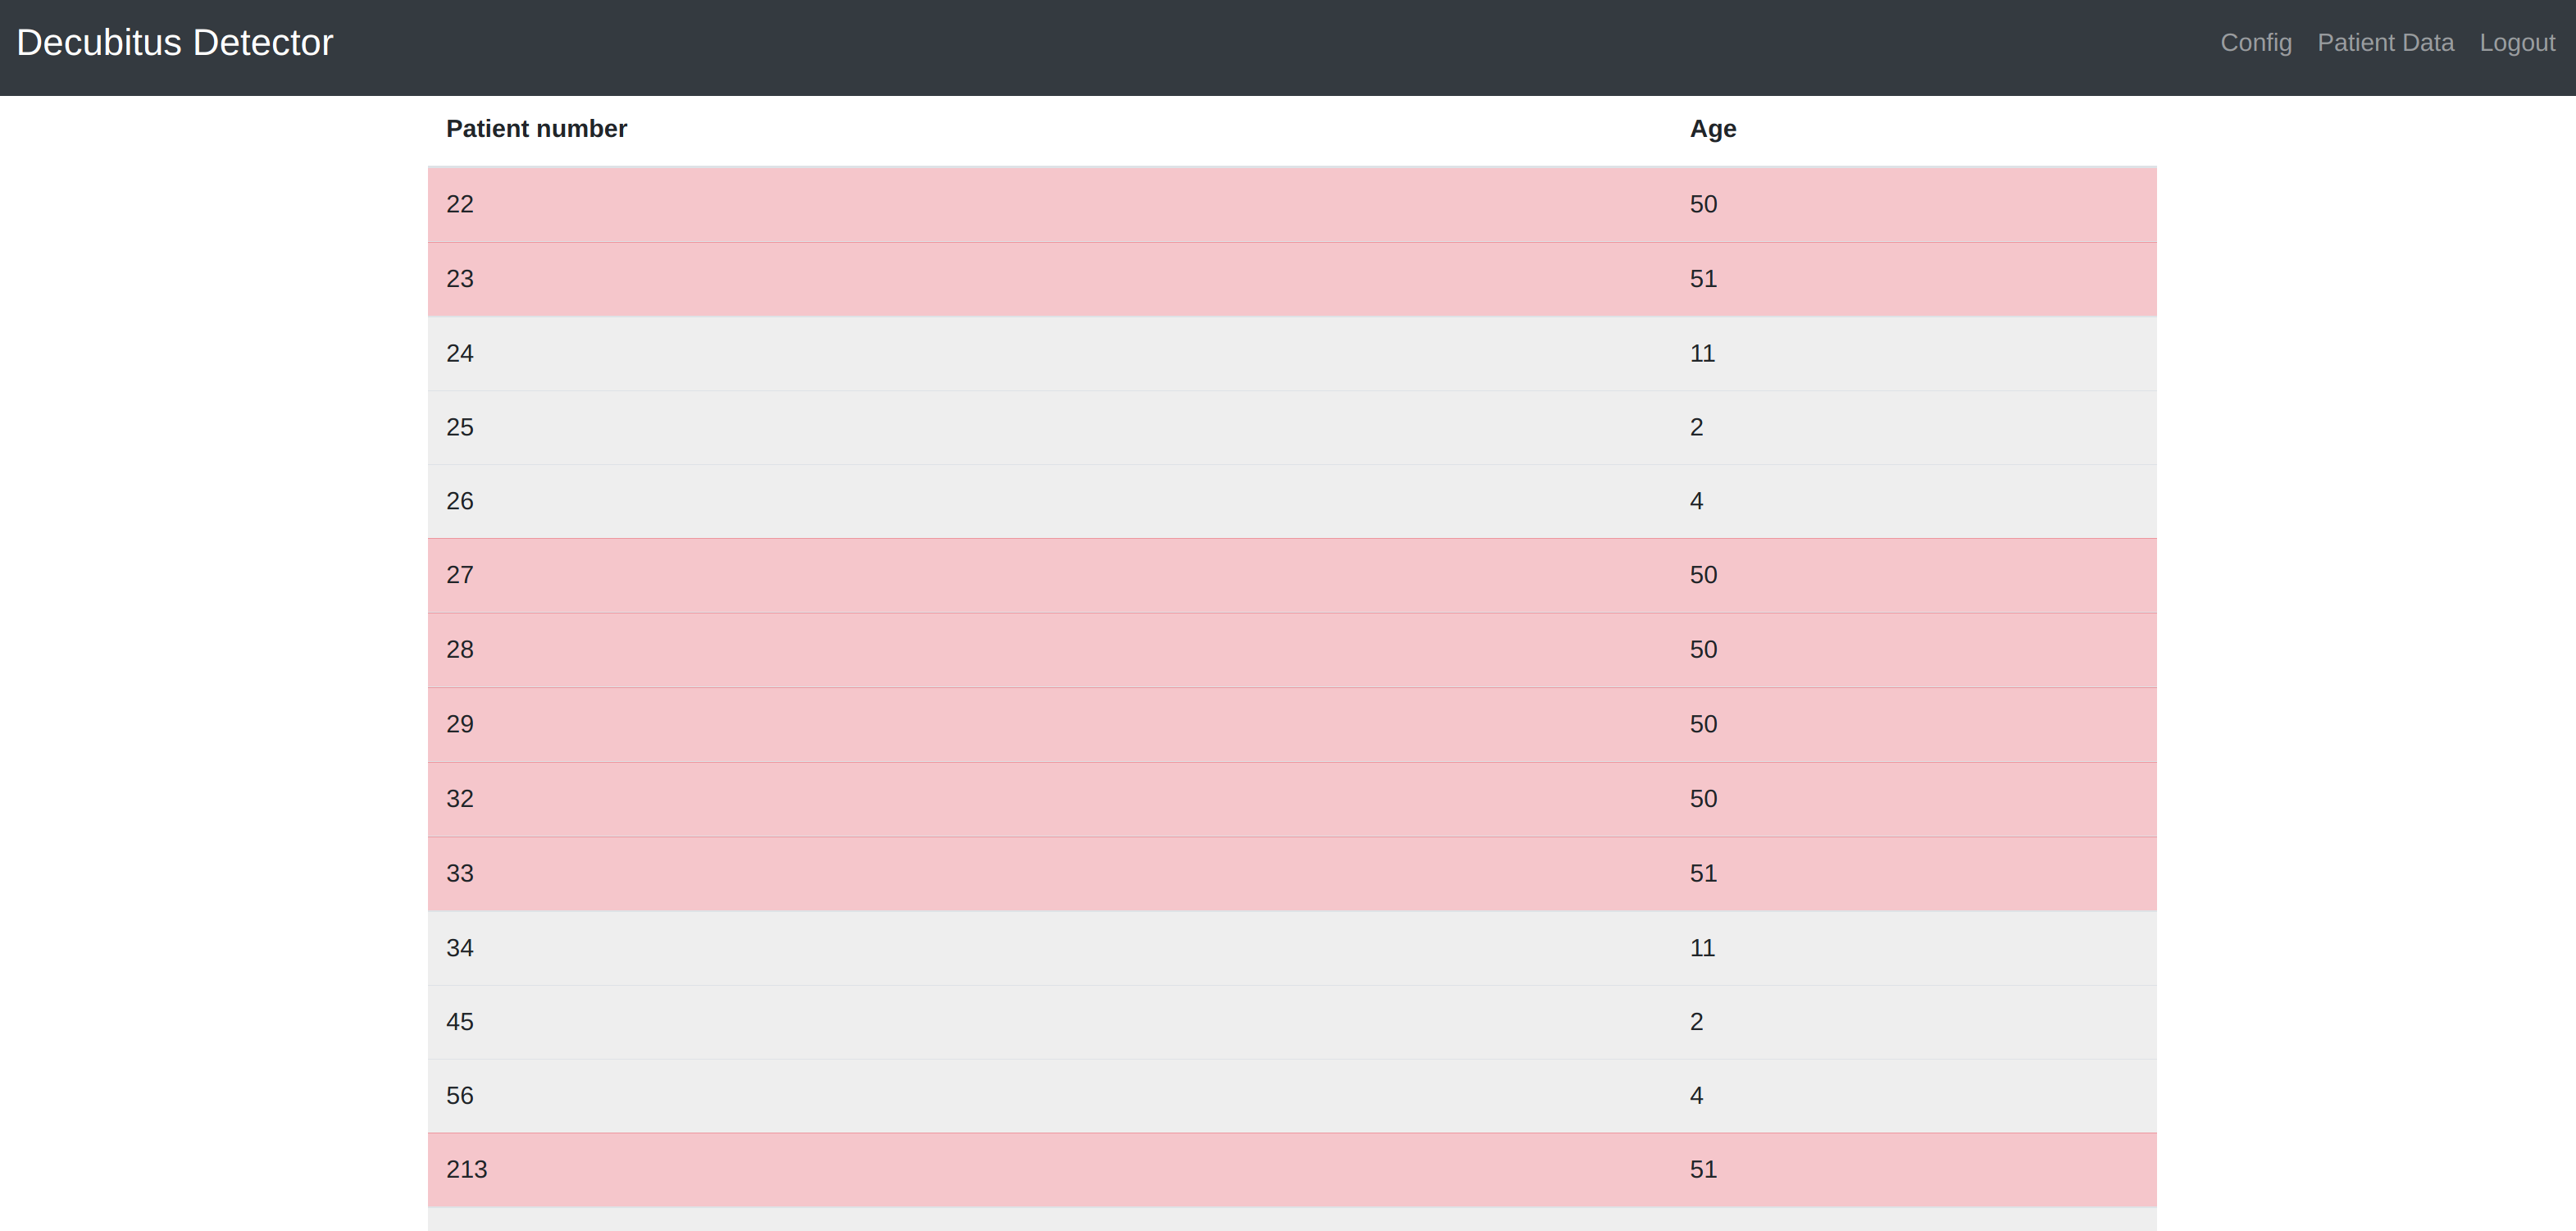
\includegraphics[width=0.8\linewidth]{images/gray.png}
	\captionsetup{labelformat=empty}
	\caption{a) Undetected patients are colorized in gray.}
  \label{fig:red}
\end{figure}

\begin{figure}[H]
	\centering
  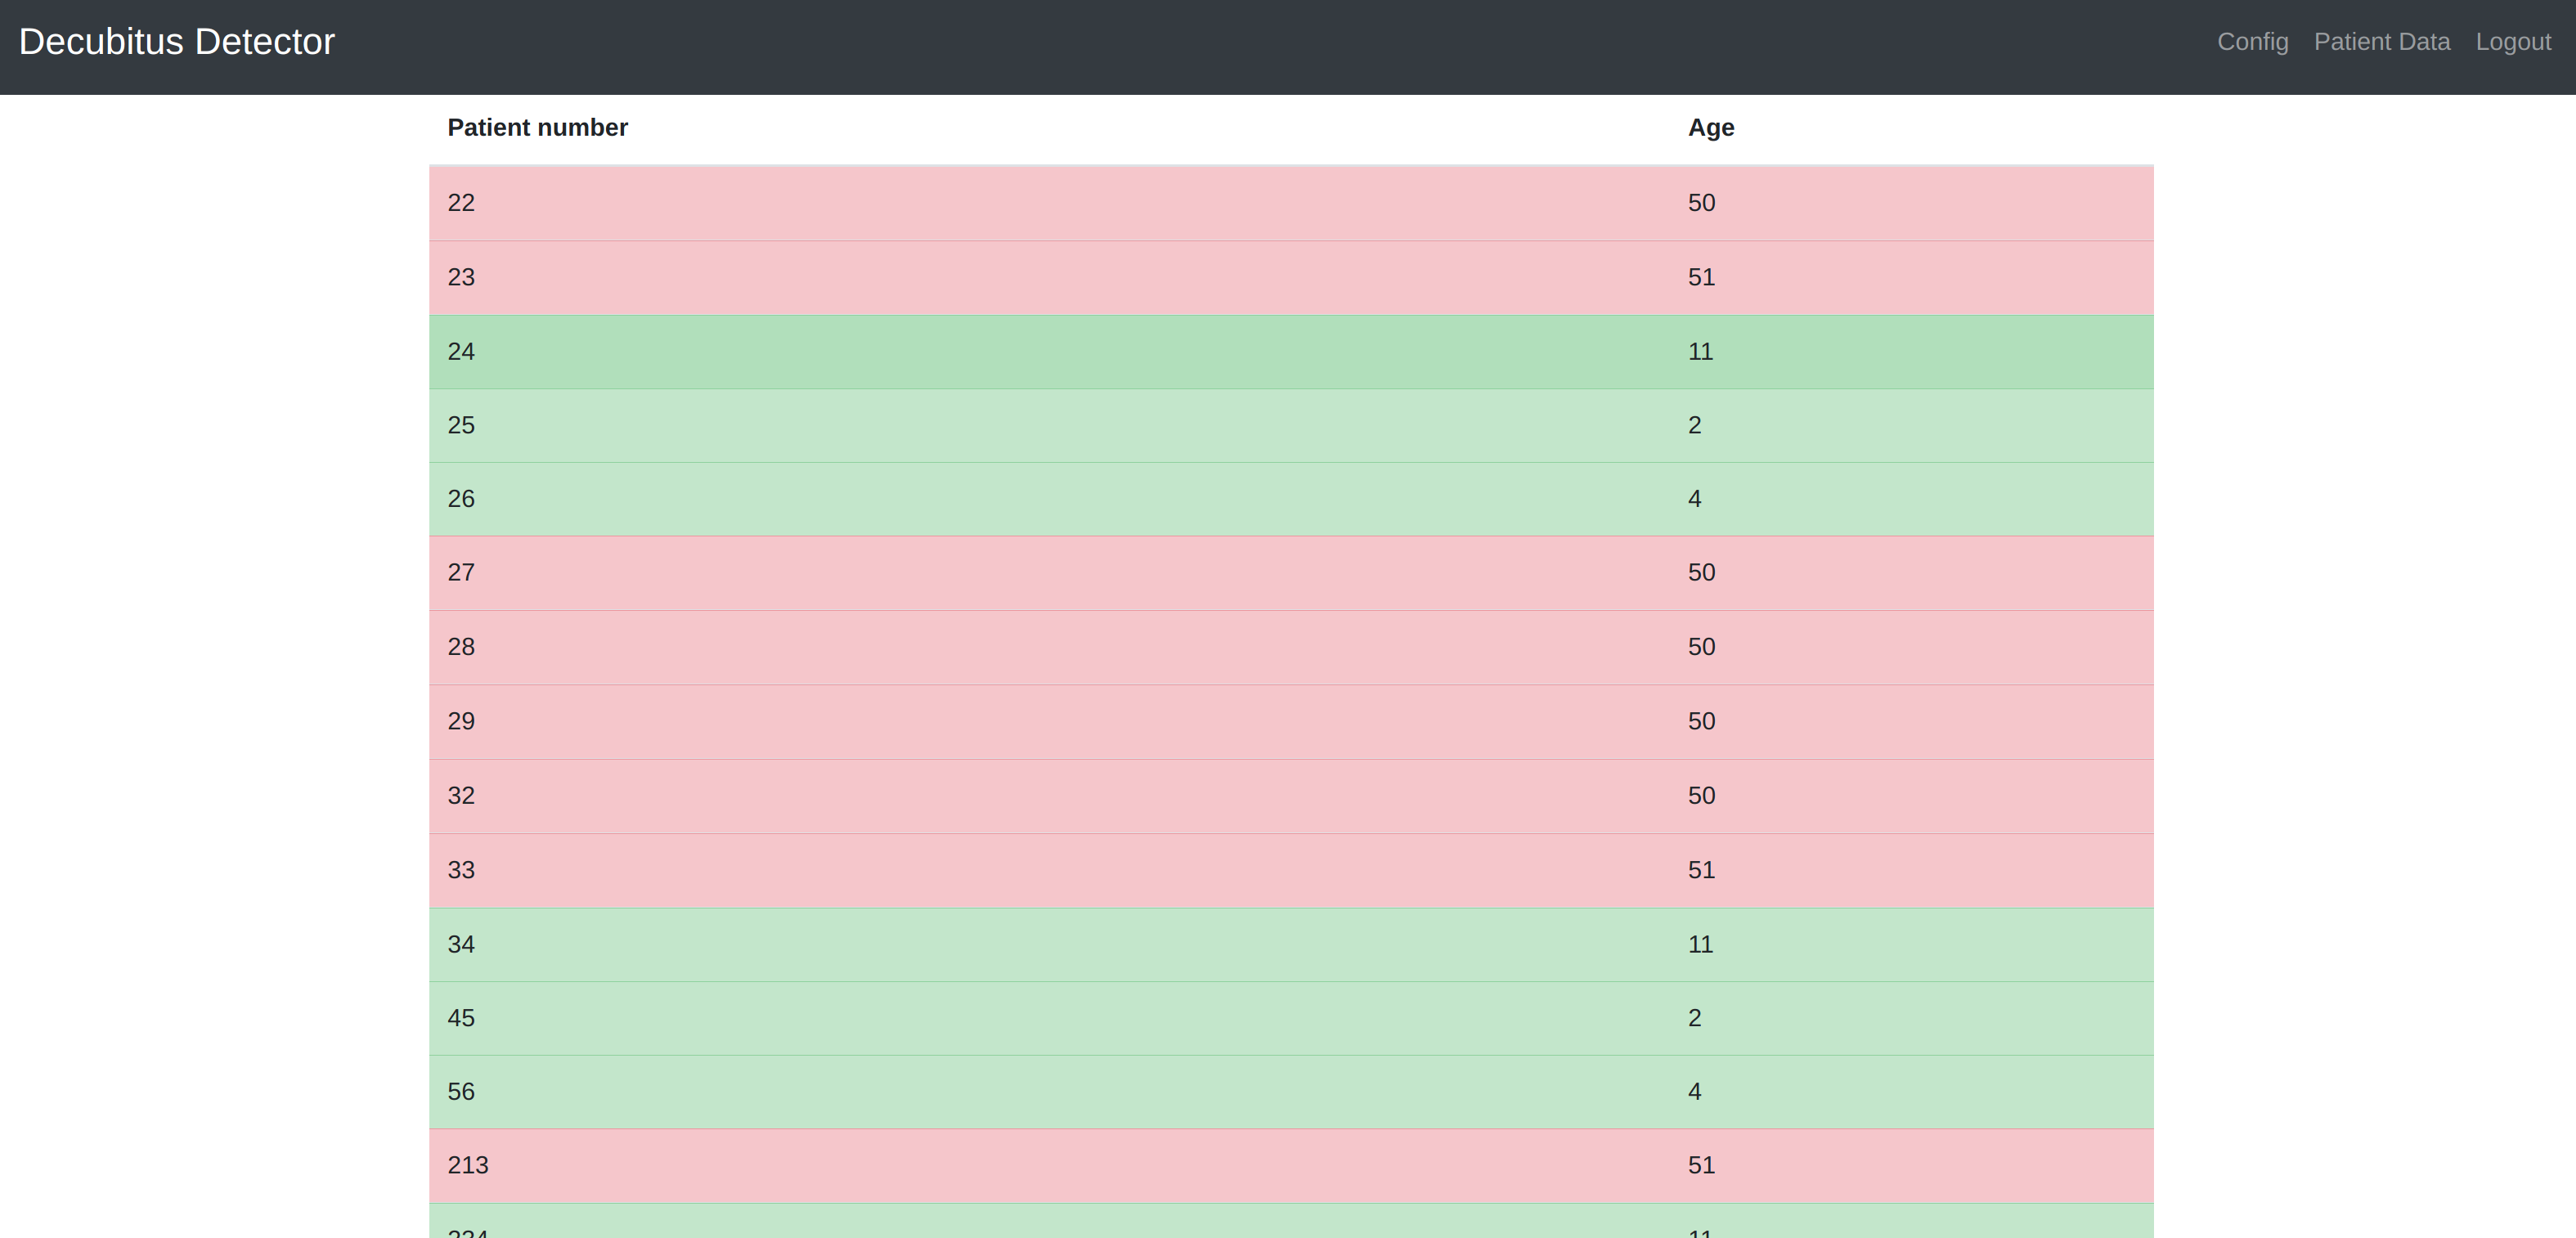
\includegraphics[width=0.8\linewidth]{images/green.png}
	\captionsetup{labelformat=empty}
	\caption{ b) Undetected patients are colorized in green.}
  \label{fig:green}
\end{figure}

\begin{figure}[H]
	\centering
  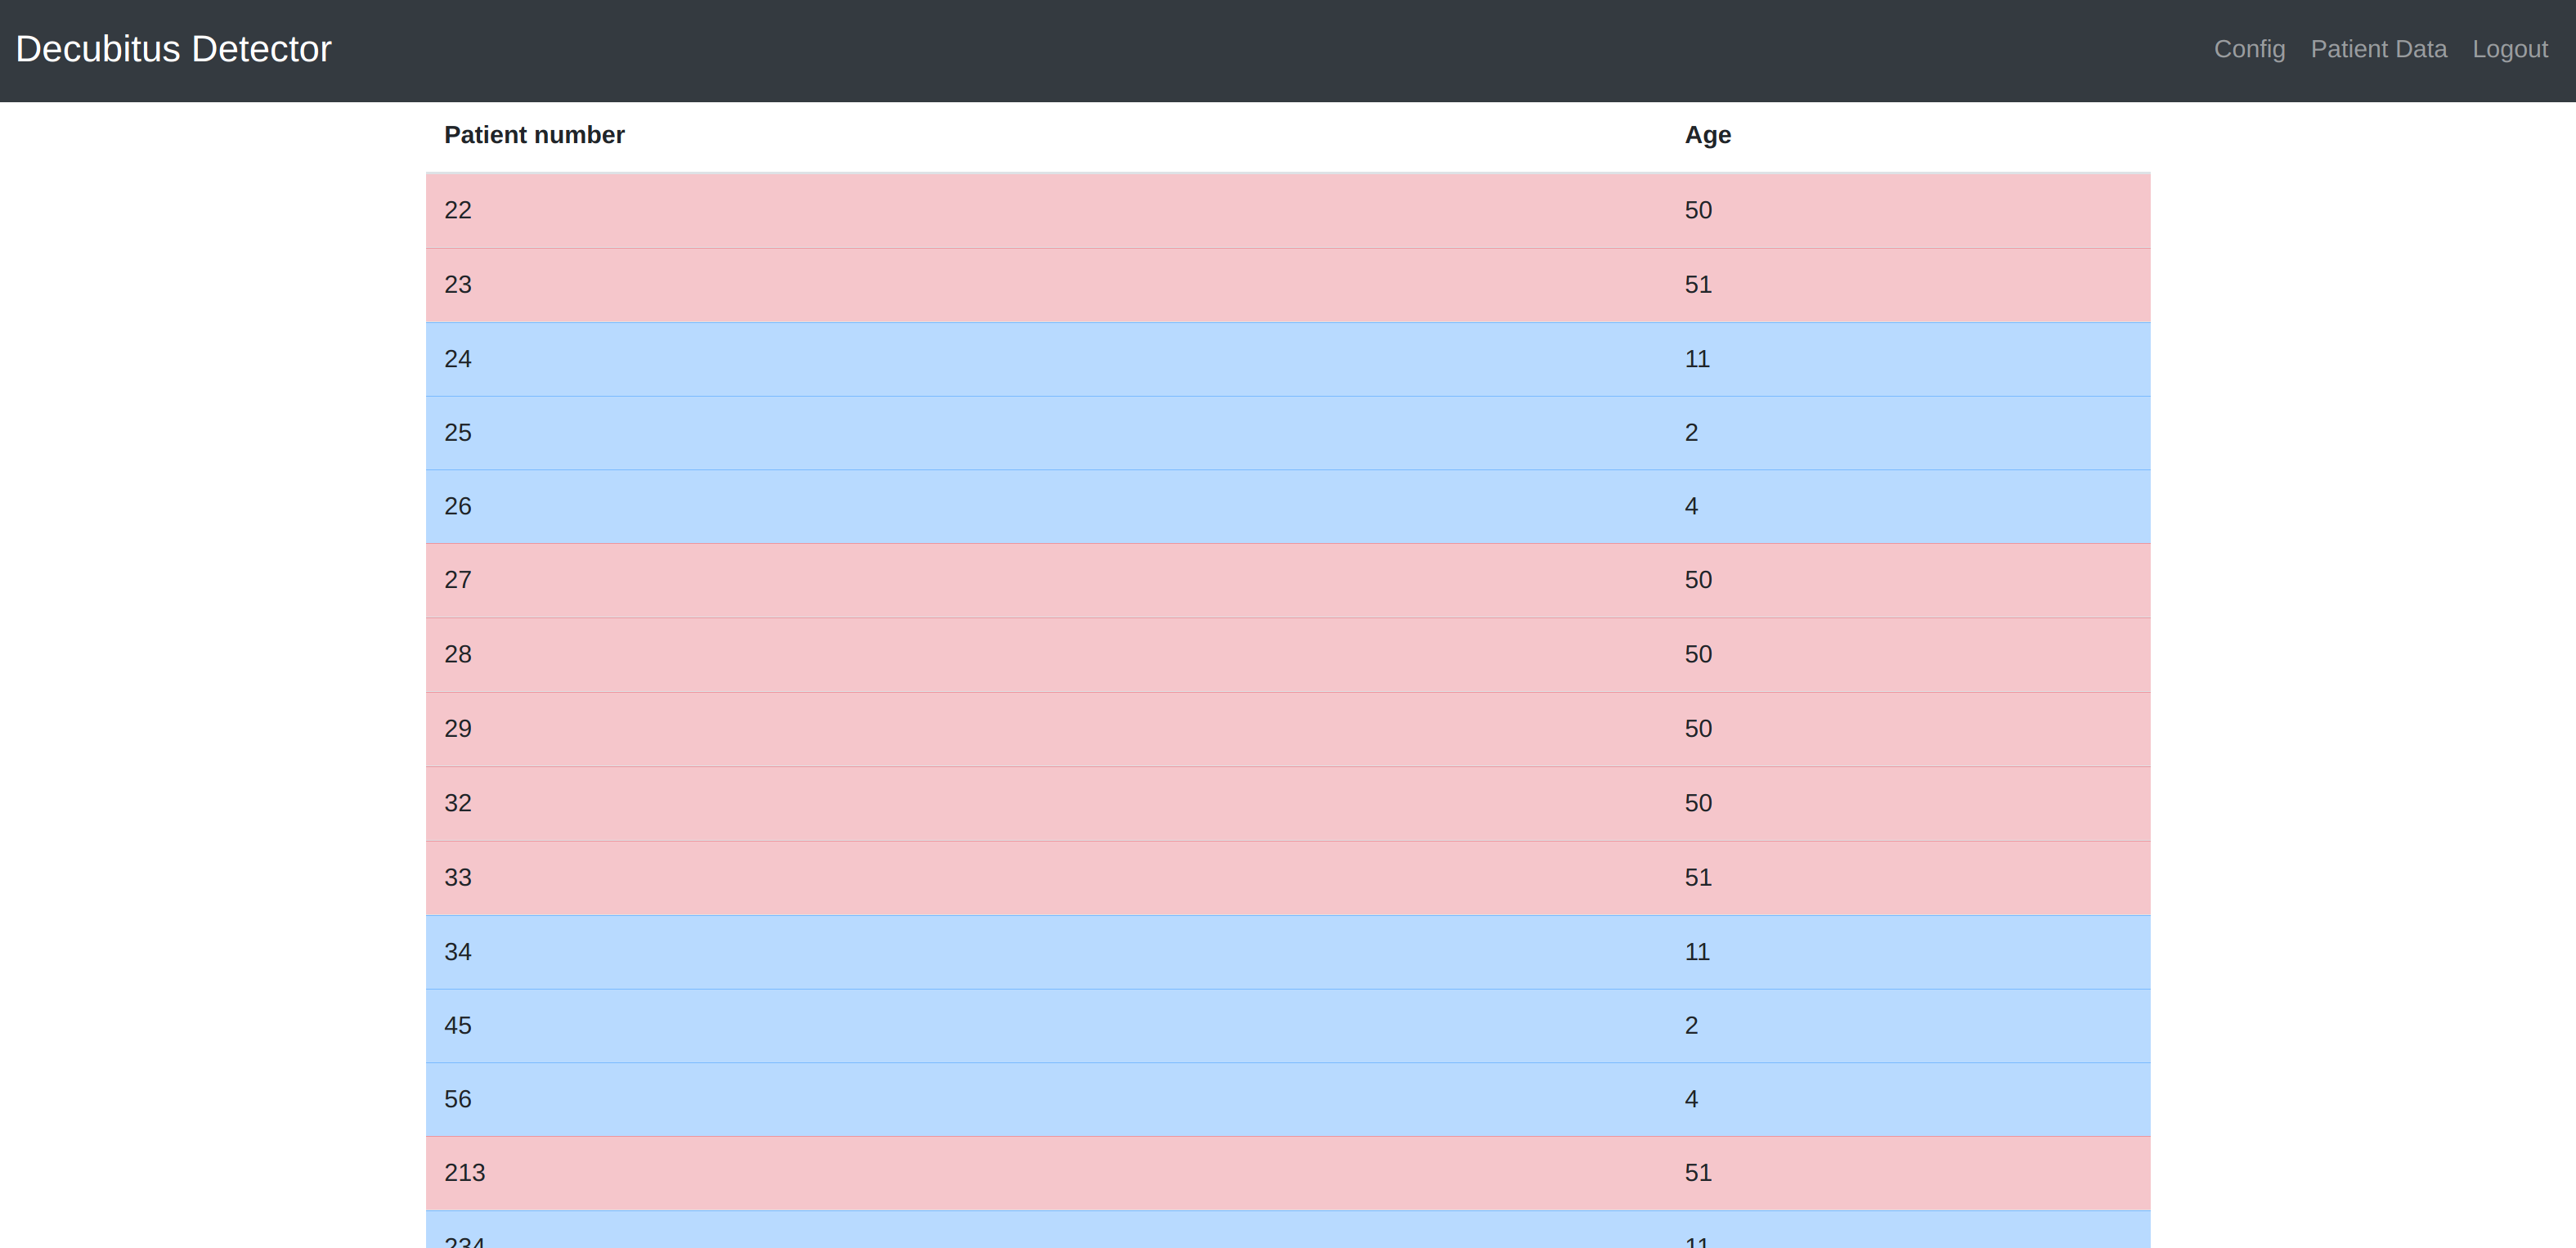
\includegraphics[width=0.8\linewidth]{images/blue.png}
	\captionsetup{labelformat=empty}
	\caption{c) Undetected patients are colorized in blue.}
  \label{fig:blue}
\end{figure}
\fi

\begin{questions}

\question Which color theme do you believe is the most suitable one?

\begin{checkboxes}
	\choice a)
	\choice b)
	\choice c)
	\choice d)
\end{checkboxes}

\end{questions}

\subsection*{Lists vs. Text}

\setcounter{eqn}{0}

The following images show the reasons, why out algorithm detected decubitus in different styles: As a list and as text. 

\begin{tabular}{cc}
	\num\putindeepbox[7pt]{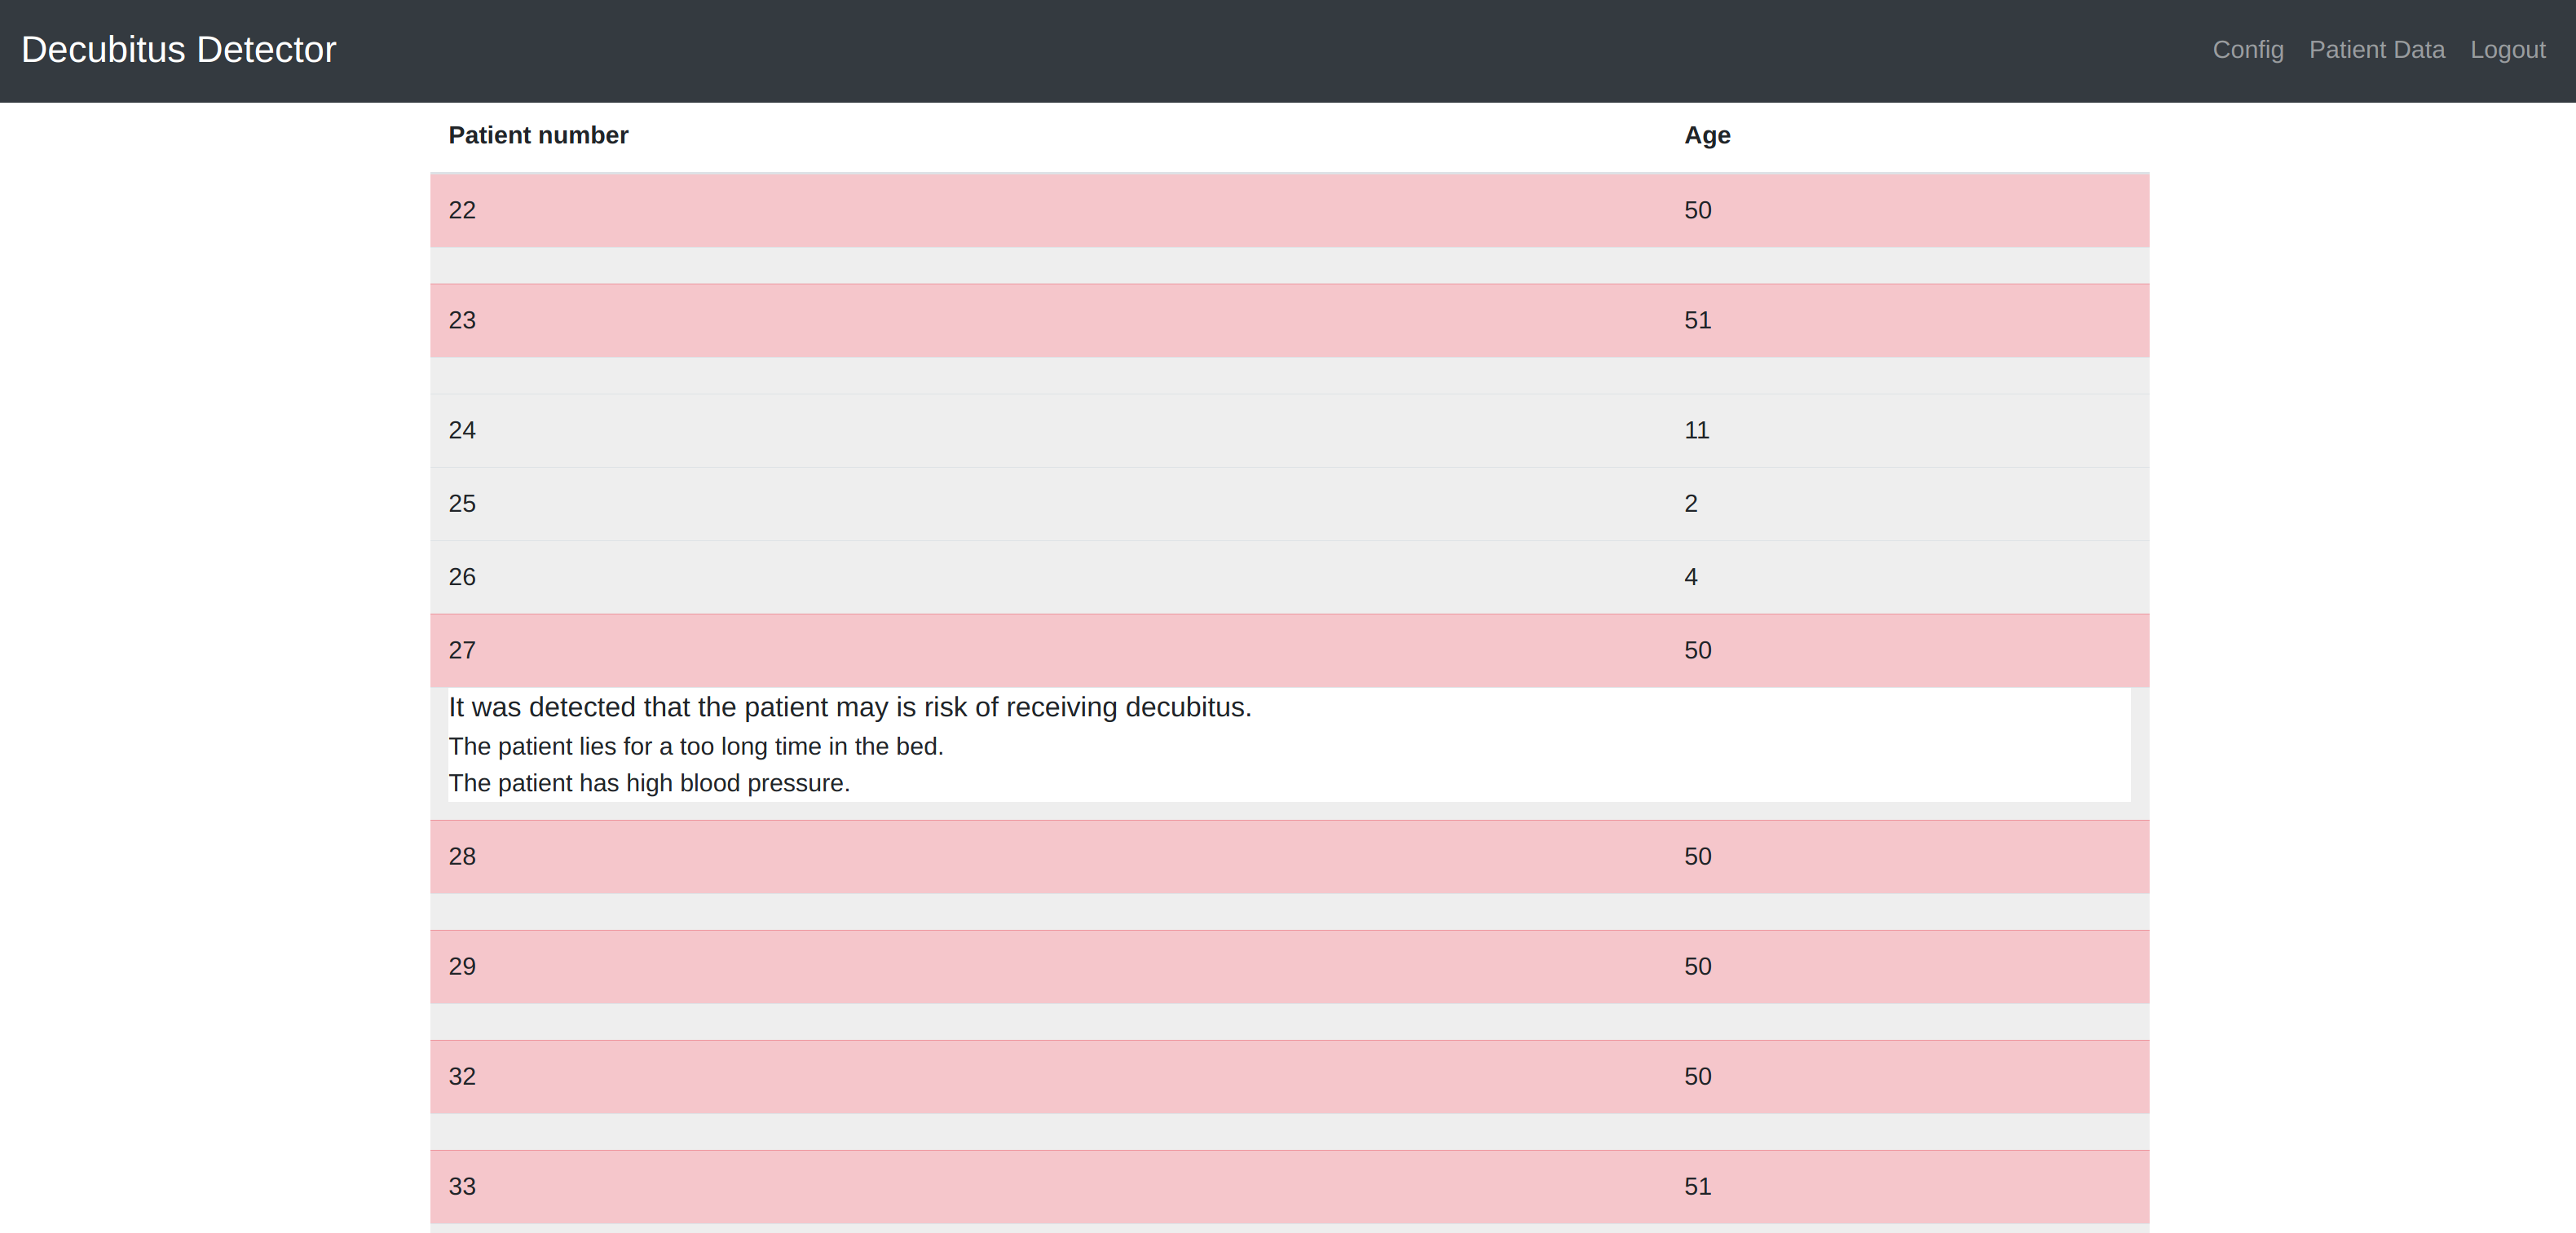
\includegraphics[width=0.45\linewidth]{images/text.png}}
	& \num\putindeepbox[7pt]{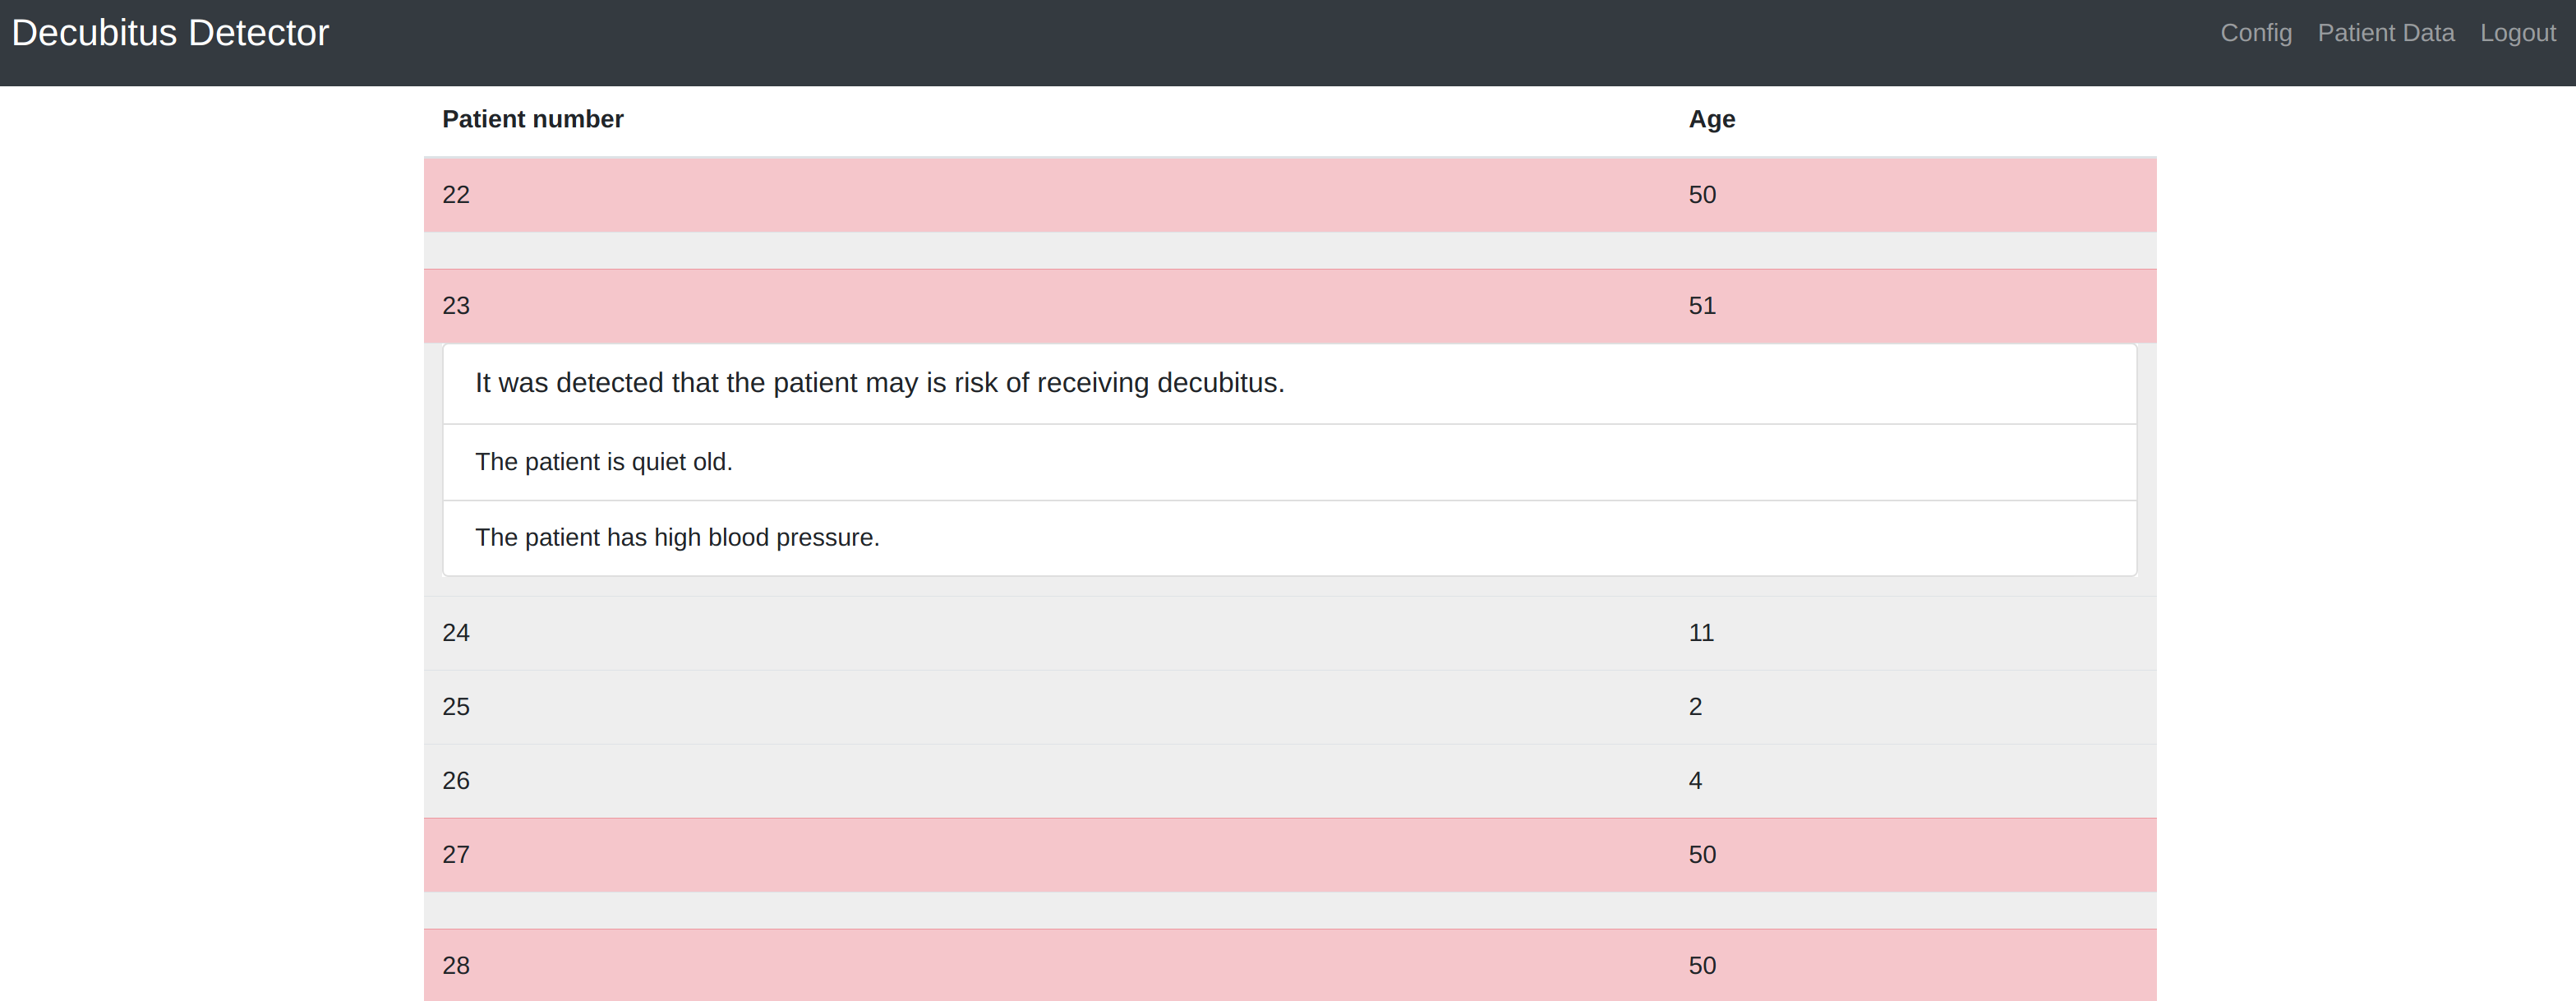
\includegraphics[width=0.45\linewidth]{images/lists.png}} \\
\end{tabular}

\iffalse
\begin{figure}[H]
	\centering
  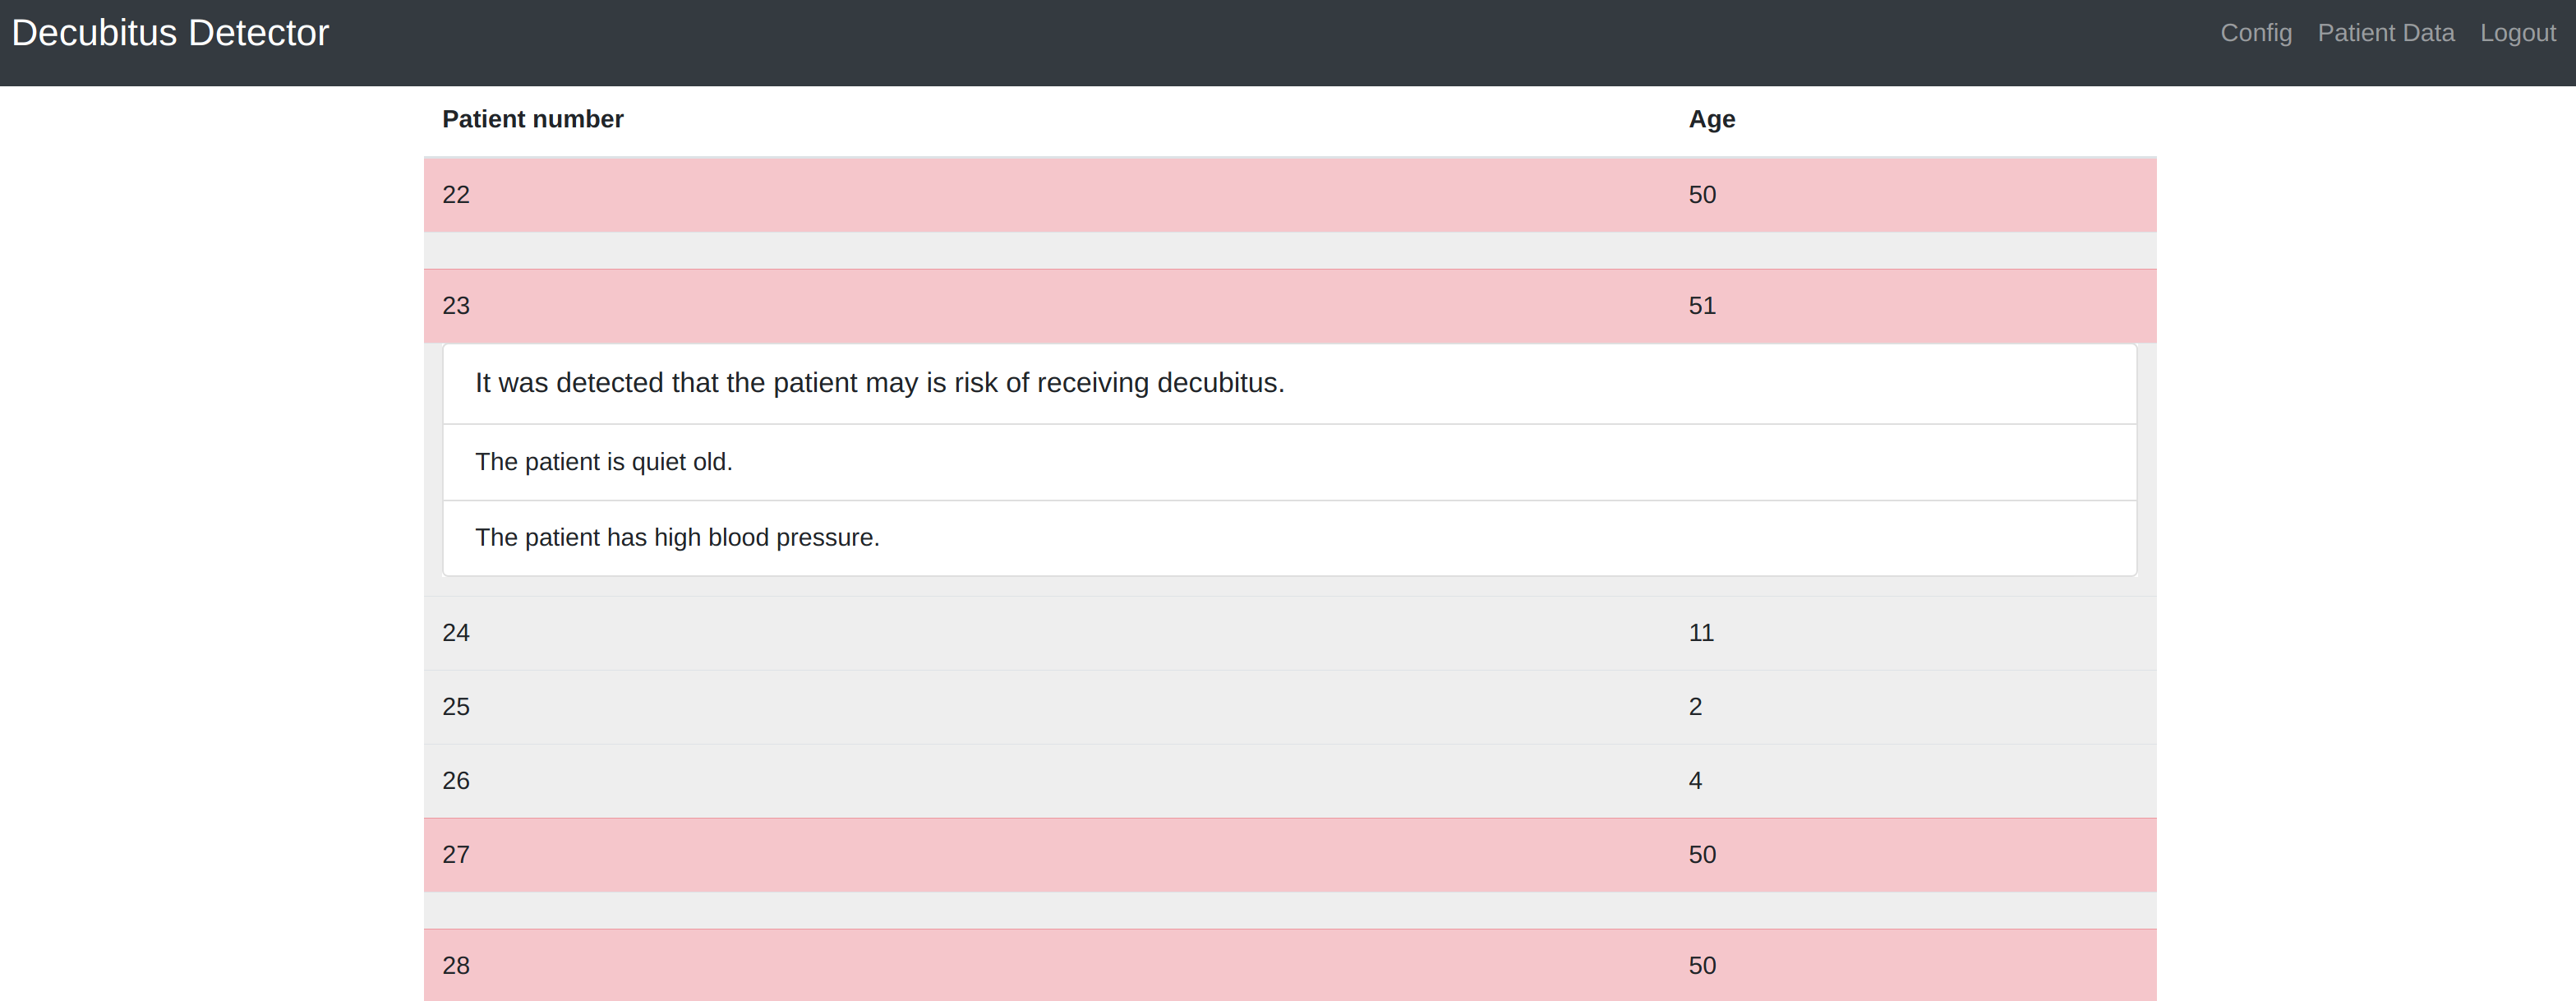
\includegraphics[width=0.8\linewidth]{images/lists.png}
	\captionsetup{labelformat=empty}
	\caption{ a) The explanation of the decision of our decision is illustrated as a list.}
  \label{fig:list}
\end{figure}

\begin{figure}[H]
	\centering
  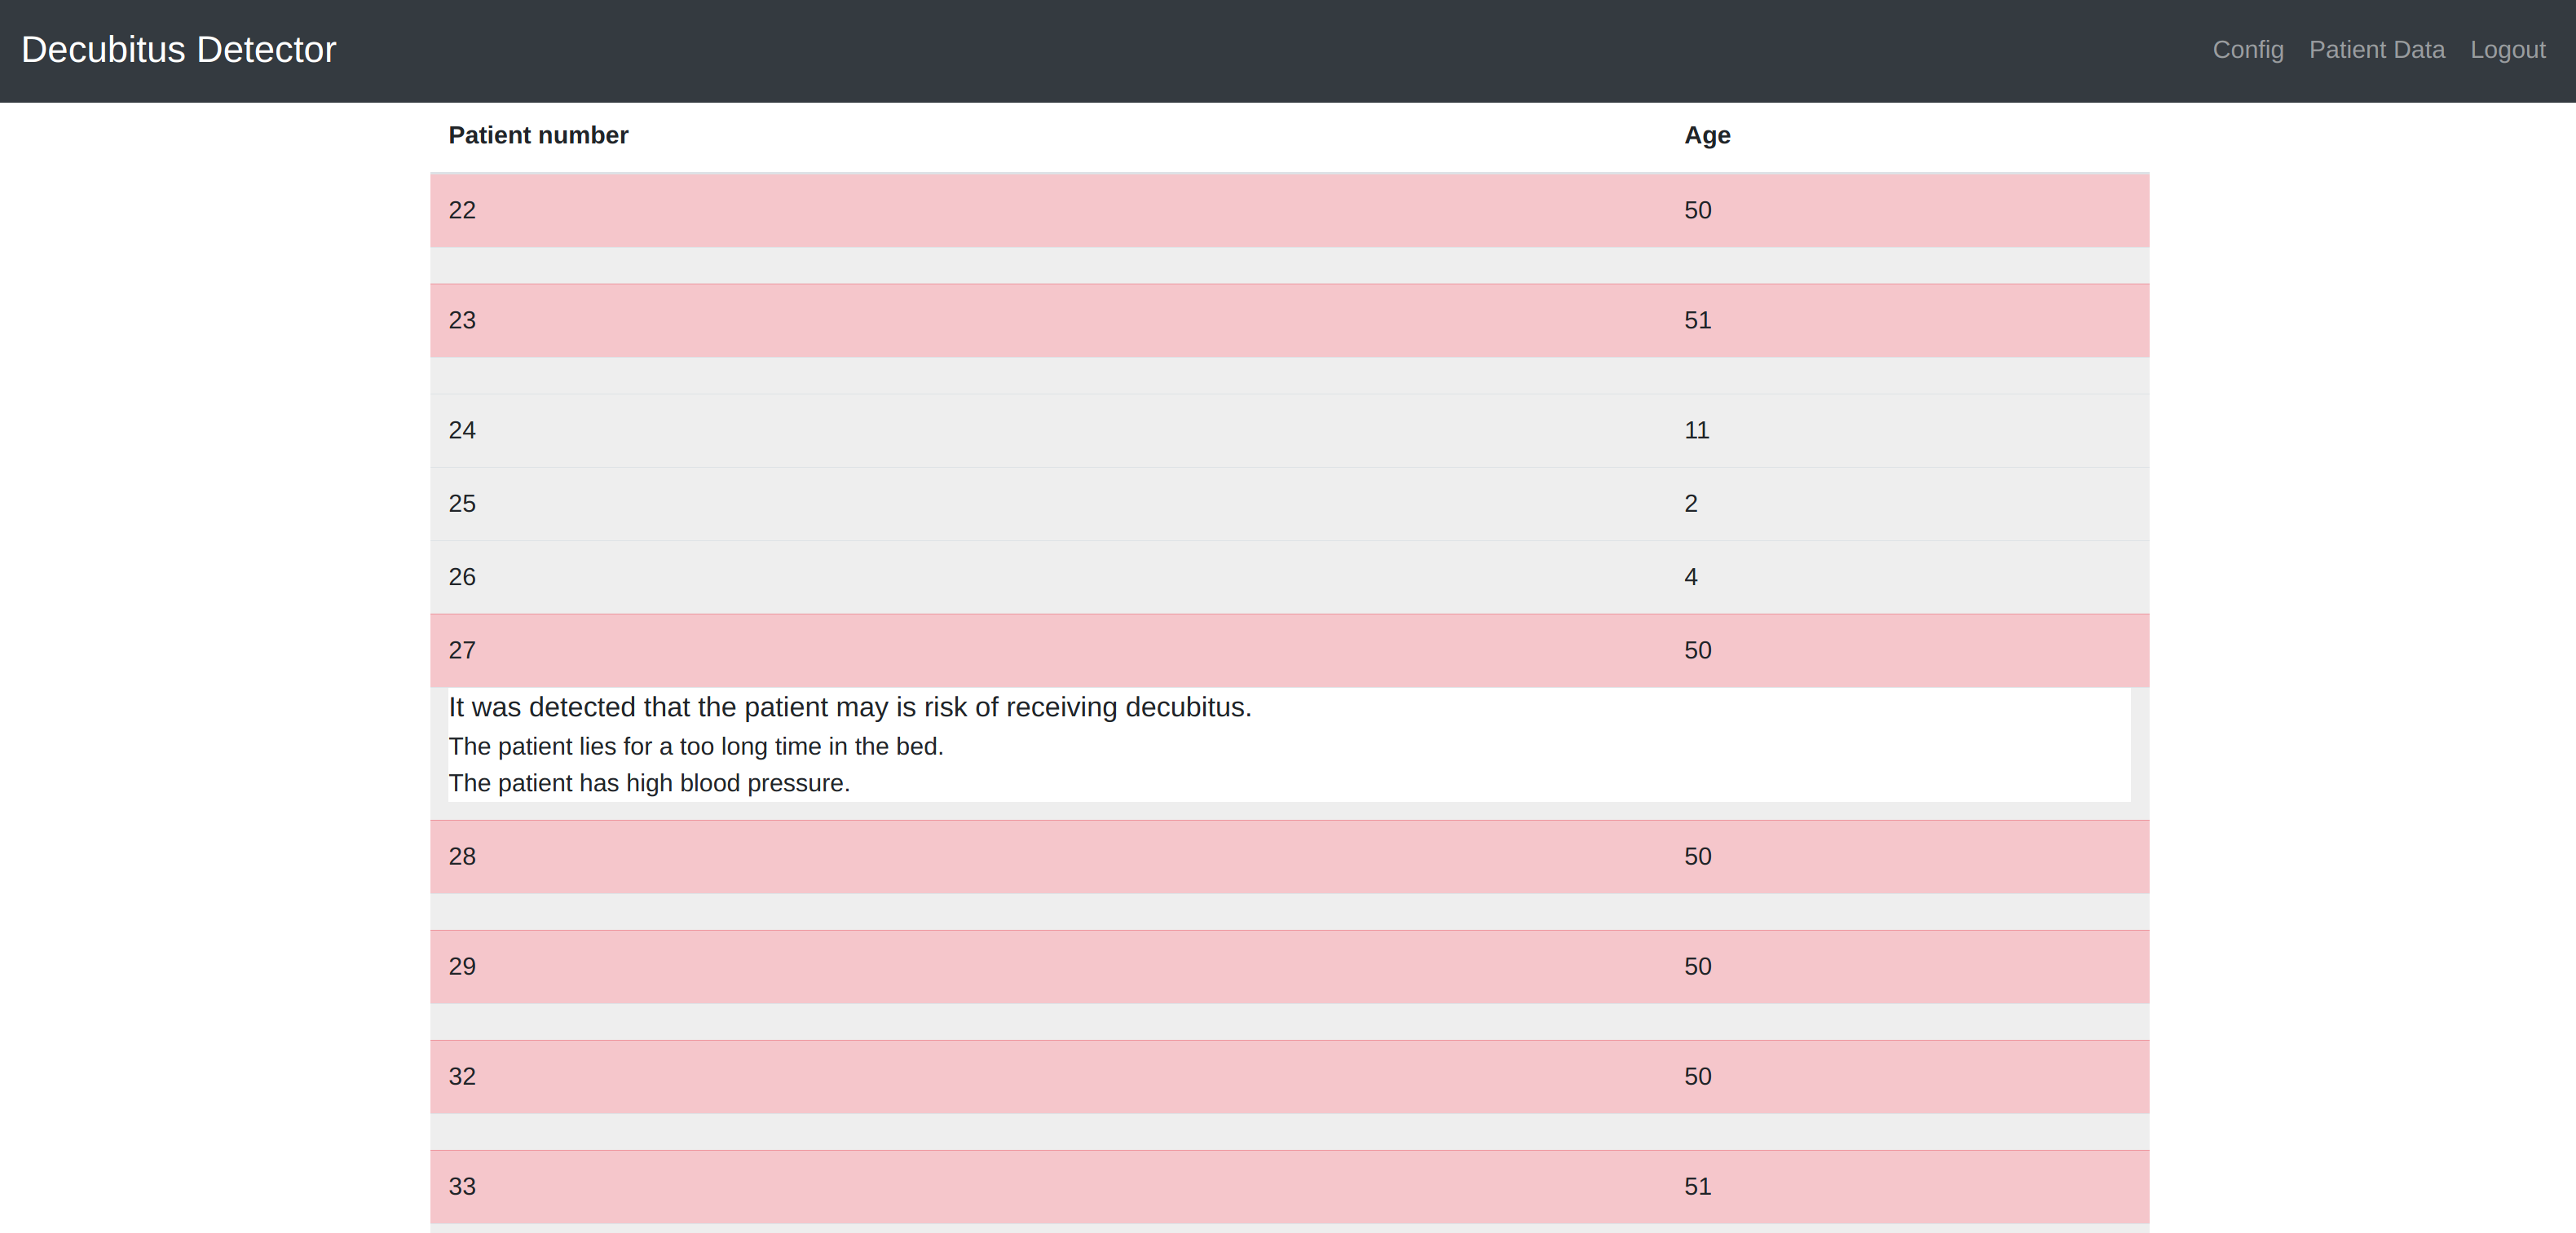
\includegraphics[width=0.8\linewidth]{images/text.png}
	\captionsetup{labelformat=empty}
	\caption{b) The explanation of the decision of the algorithm is illustrated as a text.}
  \label{fig:text}
\end{figure}
\fi

\begin{questions}

\question Would you prefer a text or a list?

\begin{checkboxes}
	\choice a)
	\choice b)
\end{checkboxes}

\end{questions}

\section*{Functionality}

\subsection*{Database Settings}

The frontend is completely separated from the ETL process and the detection algorithm. It just shows the results from the database. 
Therefore the database settings must be configured. By assumption, most doctors will be confused with this task. Should we still give him the option to 
do change the database connection settings? The following image shows how the configuration page looks like. 
Note: As the frontend is basically a website, a server admin should still be able to modify the settings.  

\begin{figure}[H]
	\centering
  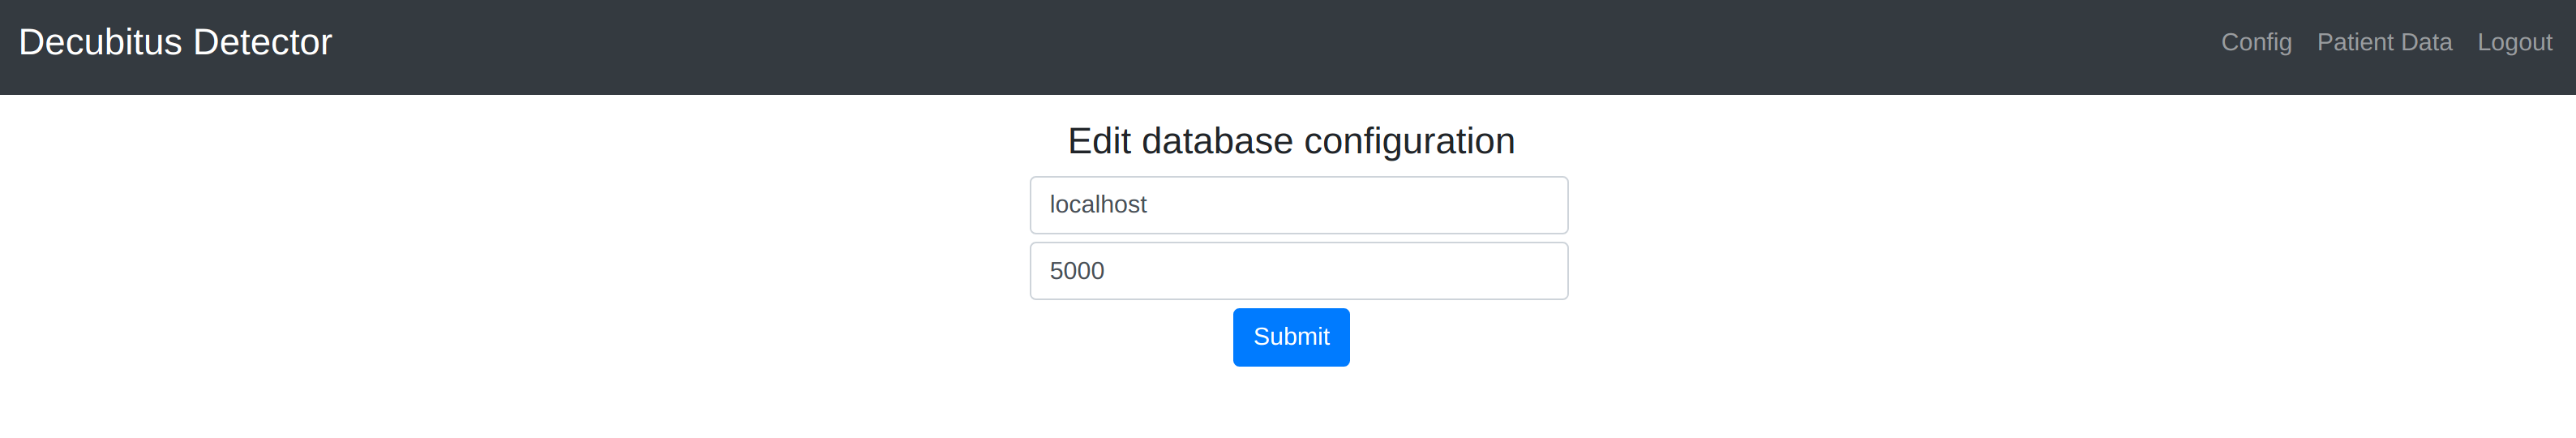
\includegraphics[width=0.8\linewidth]{images/db.png}
	\captionsetup{labelformat=empty}
	\caption{The config page.}
  \label{fig:text}
\end{figure}

\begin{questions}
\question Would you give the doctor the option to modify the database settings?

\begin{checkboxes}
	\choice Yes
	\choice No
	\choice Doesn't matter
\end{checkboxes}

\end{questions}

\subsection*{Patient Content}

Apart from reasons, why a patient is endangered, a doctor requires additional information (e.g. the patient id). 

\begin{questions}
\question Is it sufficient to show to show the ID of the patient along with his birth date?

\begin{checkboxes}
	\choice Yes
	\choice No
	\choice Doesn't matter
\end{checkboxes}

If you checked: "No", which additional information would you show the user?
\vspace{5cm}

\question Should there be an option to export the results as PDF file?

\begin{checkboxes}
	\choice Yes
	\choice No
	\choice Doesn't matter
\end{checkboxes}

\end{questions}

\subsection*{Credentials}

Medical records are highly confidential. One can prevent leaking data by a authentication system. The following image shows a login page.

\begin{figure}[H]
	\centering
  
\includegraphics[width=0.8\linewidth]{images/login.png}
	\captionsetup{labelformat=empty}
	\caption{The login page.}
  \label{fig:text}
\end{figure}

\begin{questions}
	\question Should we include the login page?

	\begin{checkboxes}
		\choice Yes
		\choice No
		\choice Doesn't matter
	\end{checkboxes}

\end{questions}

\end{document}
